\subsection{Ejercicio 14}
\graphicspath{ {img/14} }

%\begin{itemize}
%    \item \href{https://support.mozilla.org/es/kb/Gestionar-la-configuraci%C3%B3n-del-almacenamiento-local-del-sitio?as=u&utm_source=inproduct&redirectslug=permission-store-data&redirectlocale=en-US}{support.mozilla.org}
%    \item \href{https://librewolf.net/docs/faq/#how-do-i-stay-logged-into-specific-websites}{support.librewolf.org}
%    \item \href{https://addons.mozilla.org/en-US/firefox/addon/cookie-autodelete/}{cookie_autodelete.org}
%    \item \href{https://privacybadger.org/}{privacybadger.org}
%\end{itemize}


\subsubsection{Configuración cookies Mozilla Firefox}

El navegador Mozilla Firefox proporciona múltiples opciones relacionadas con la gestión de cookies [support.mozilla.org]. Entre ellos, se destacan: 

\paragraph{Acceder a los ajustes de almacenamiento del sitio }

Esta opción permite ver y gestionar qué datos (cookies y caché) guarda cada sitio web en el navegador. Para ello, el usuario debe acceder al apartado de preferencias dentro del menú de Firefox. Una vez ahí, como se ve en la \ref{fig: opcion1_ej14} en el apartado de privacidad y seguridad se puede ver información acerca de las cookies del sitio. 

\begin{figure}[H]   
    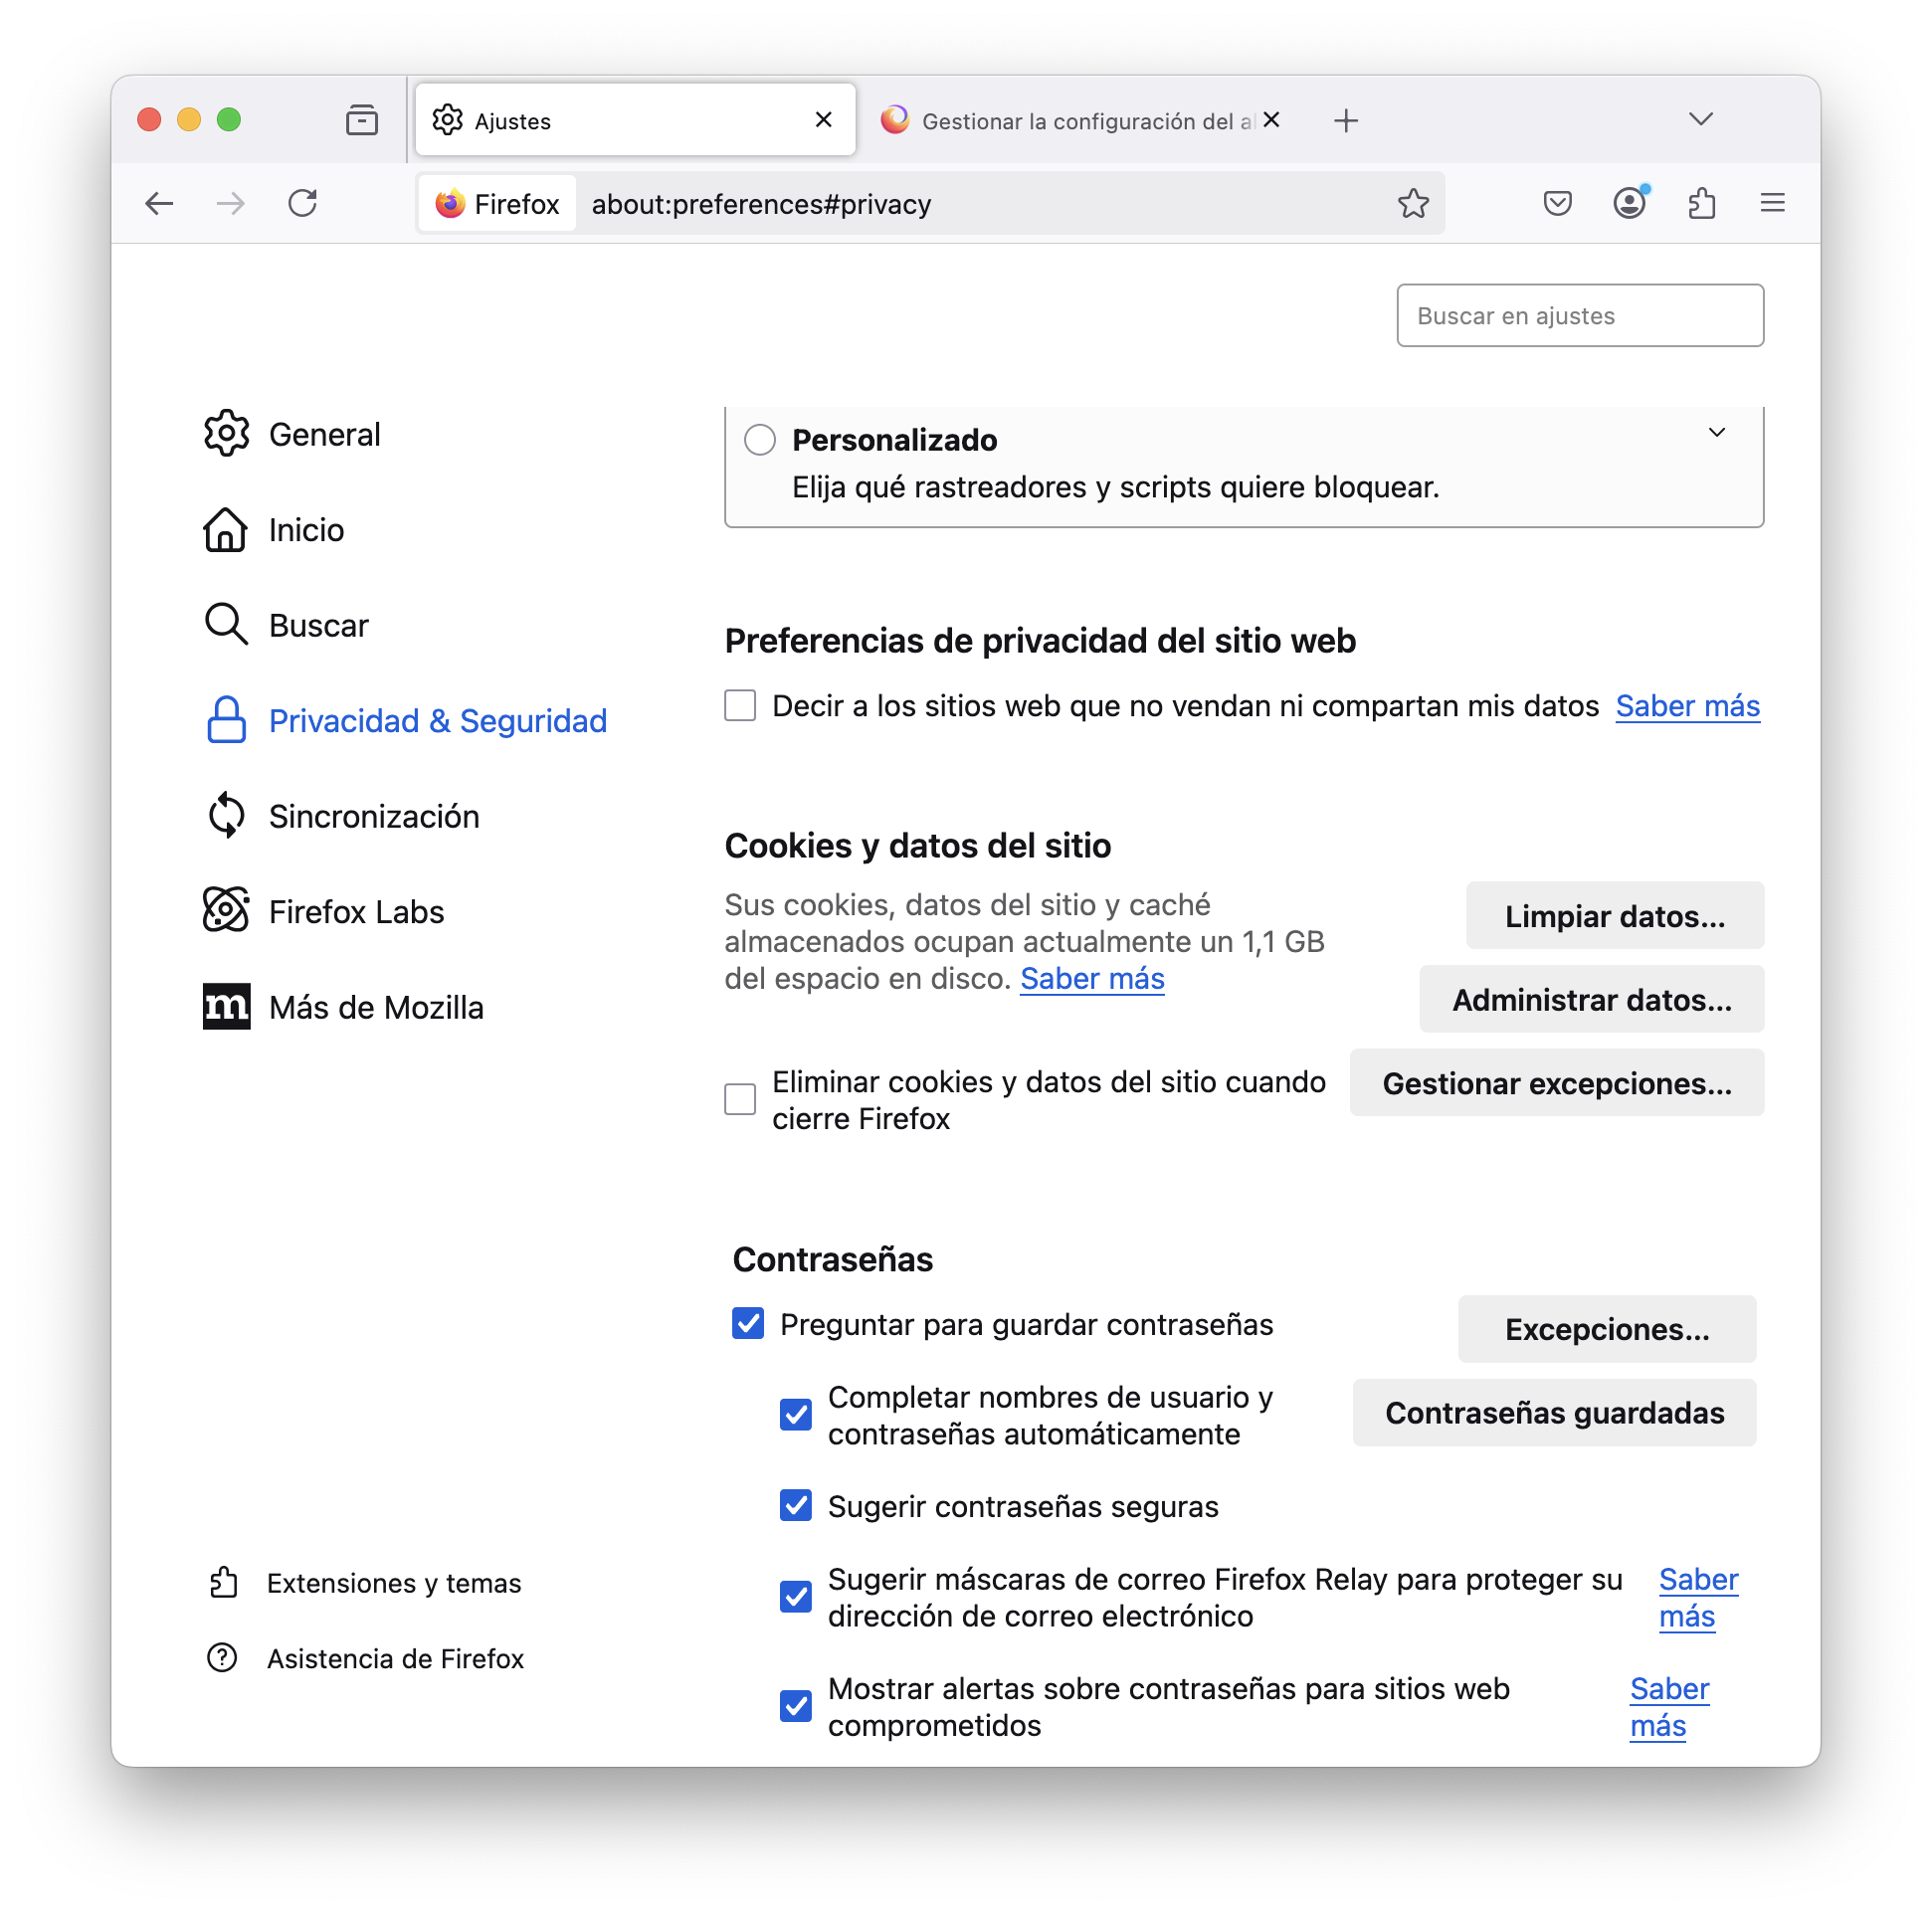
\includegraphics[width=\textwidth]{opcion1_ej14.png}
    \caption{Opción 1 de configuración de cookies, Firefox}
    \label{fig:opcion1_ej14}
\end{figure}


\paragraph{Eliminar almacenamiento del sitio en páginas individuales }

Esta opción borra los datos almacenados (como cookies) de una página web específica sin afectar a otras. Para poder aprovecharla, una vez estamos en la situación de que se muestra en la \ref{fig: opcion1_ej14} debemos seleccionar la opción "Administrar datos". Como se ve en la \ref{fig: opcion2_ej14}, aparecerá una lista de sitios y cuanta información almacena en el equipo del usuario. Ahí se podrá seleccionar el sitio que se desee para eliminar todas las cookies y datos almacenados. 

\begin{figure}[H]   
    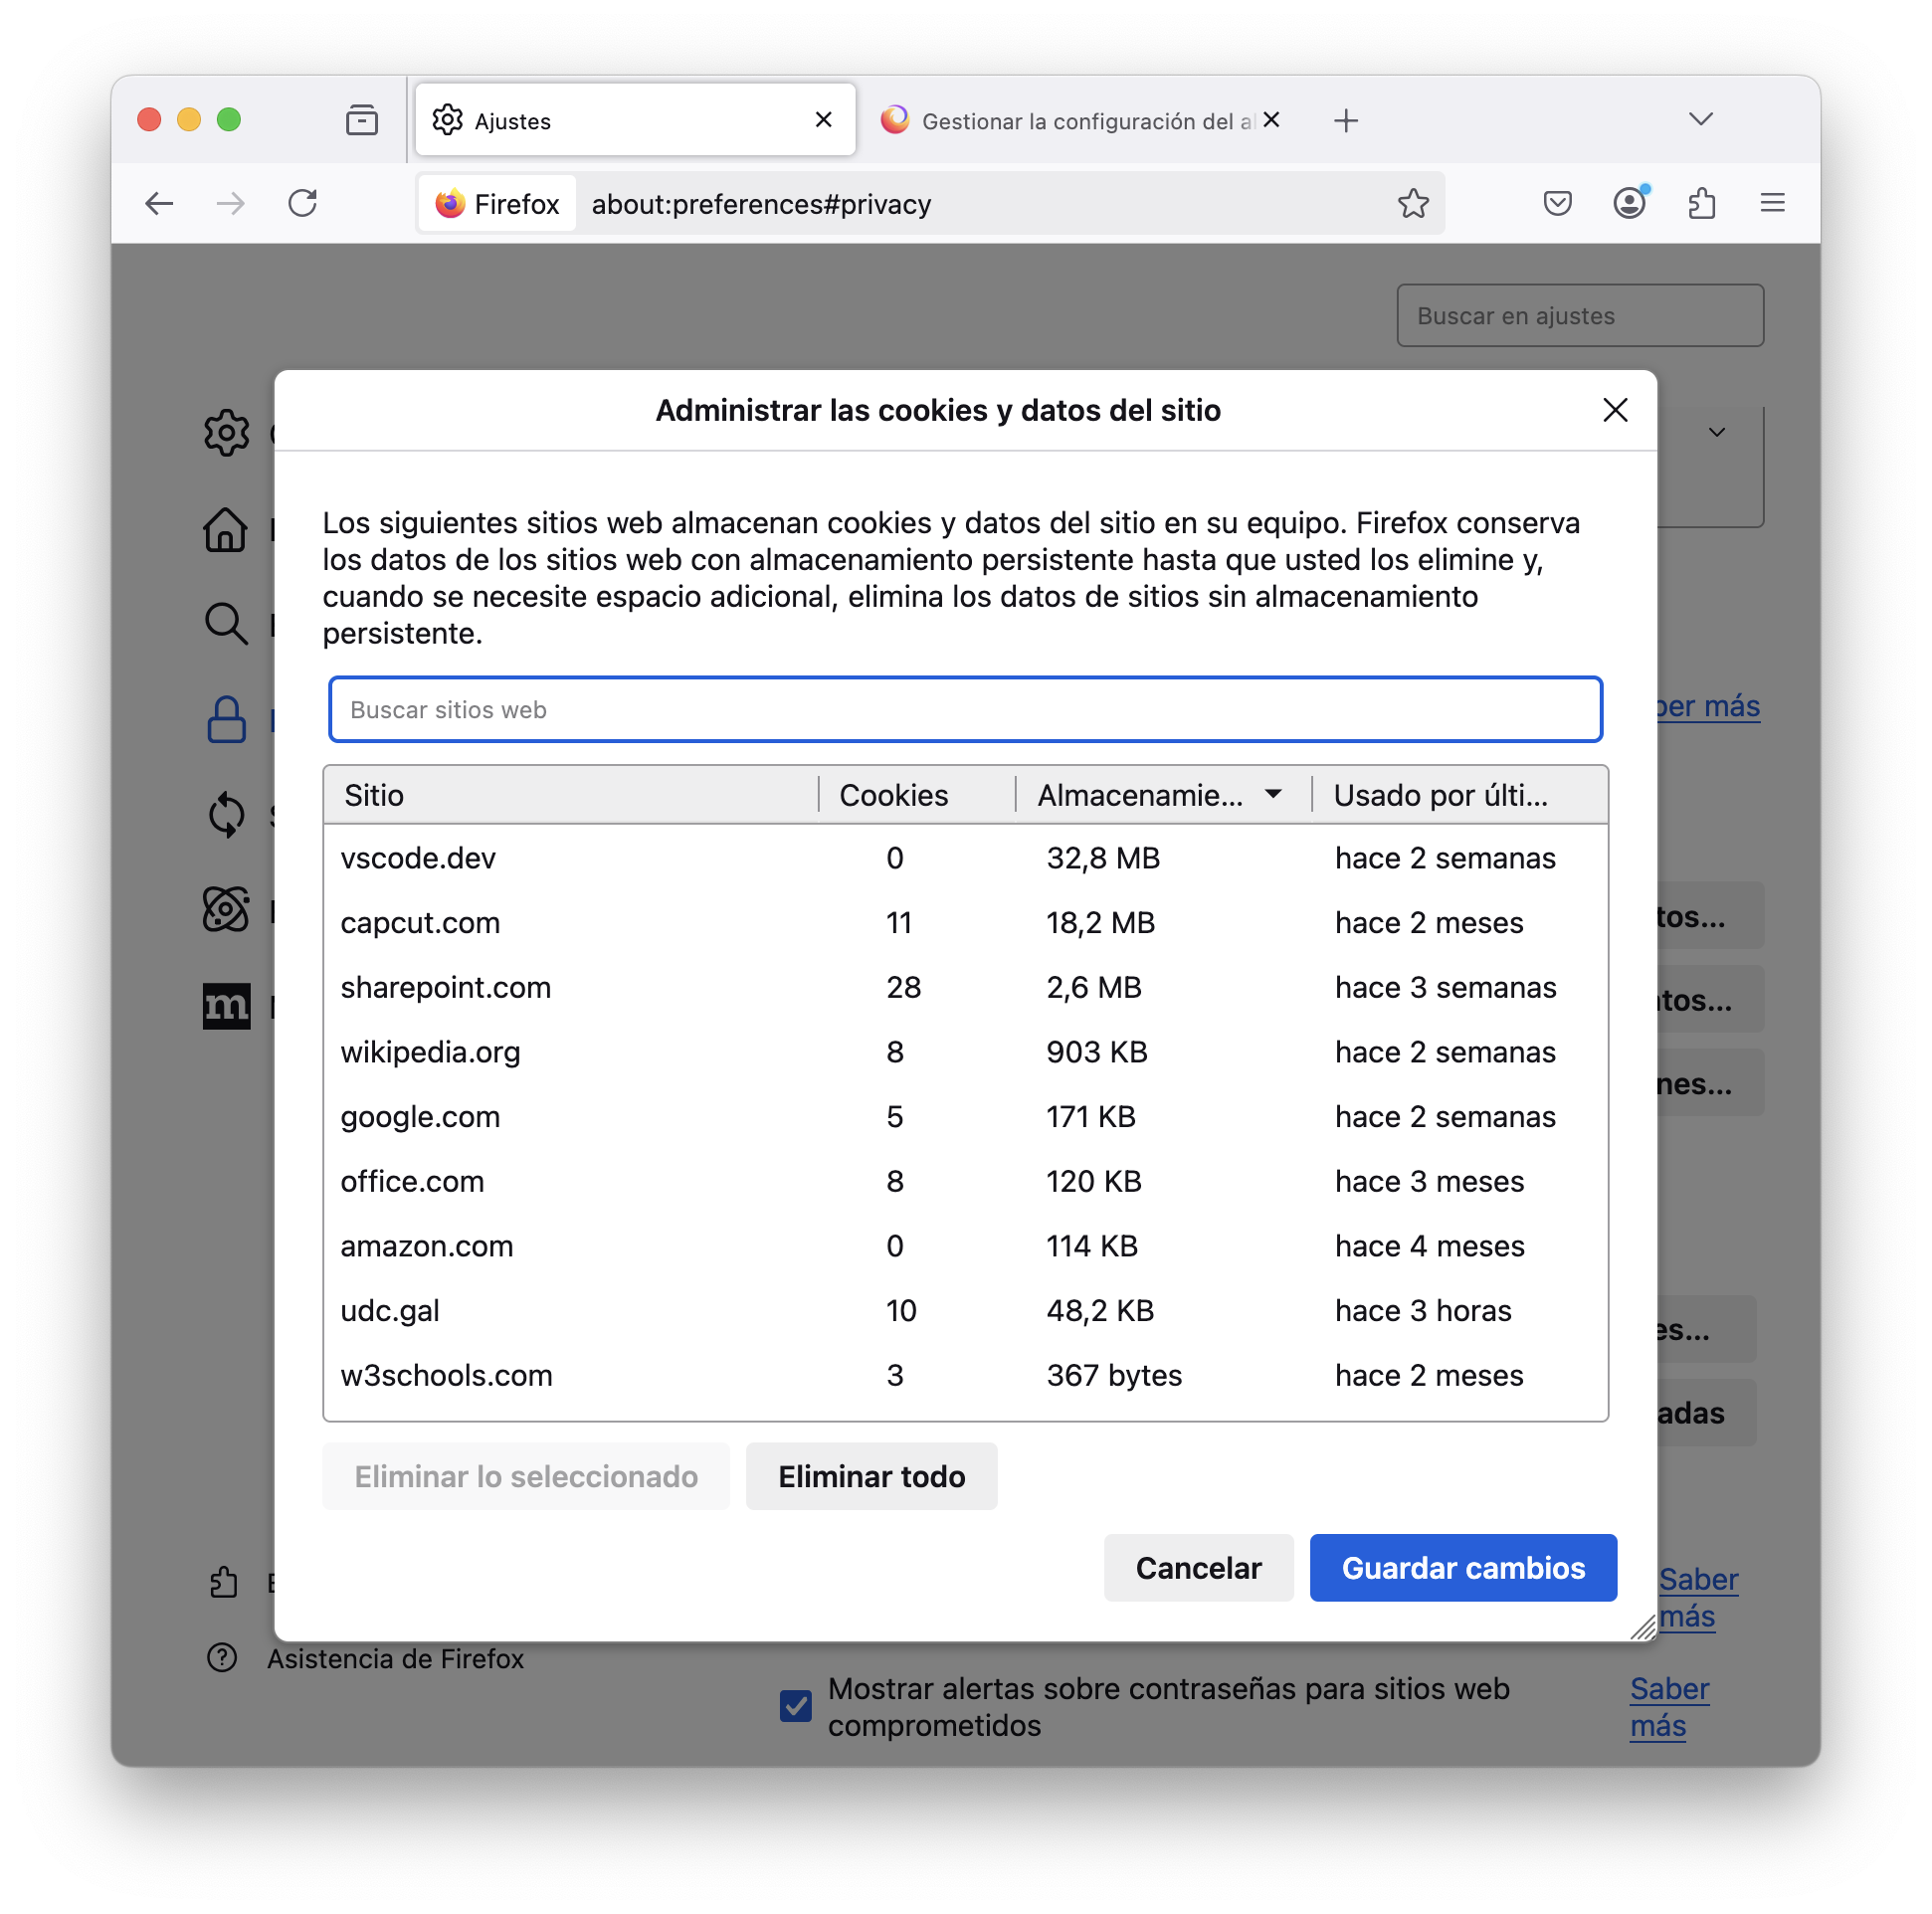
\includegraphics[width=\textwidth]{opcion2_ej14.png}
    \caption{Opción 2 de configuración de cookies, Firefox}
    \label{fig:opcion2_ej14}
\end{figure}

\paragraph{Eliminar los datos almacenados de todos los sitios}

Esta opción elimina todas las cookies y datos guardados de todos los sitios web visitados. Para poder aprovecharla, una vez estamos en la situación de que se muestra en la \ref{fig: opcion1_ej14}, debemos seleccionar la opción “Limpiar datos”. Como se ve en la \ref{fig: opcion3_ej14} se nos permite limpiar información de “cookies y datos del sitio” o “contenido de caché", entre otras. 

\begin{figure}[H]   
    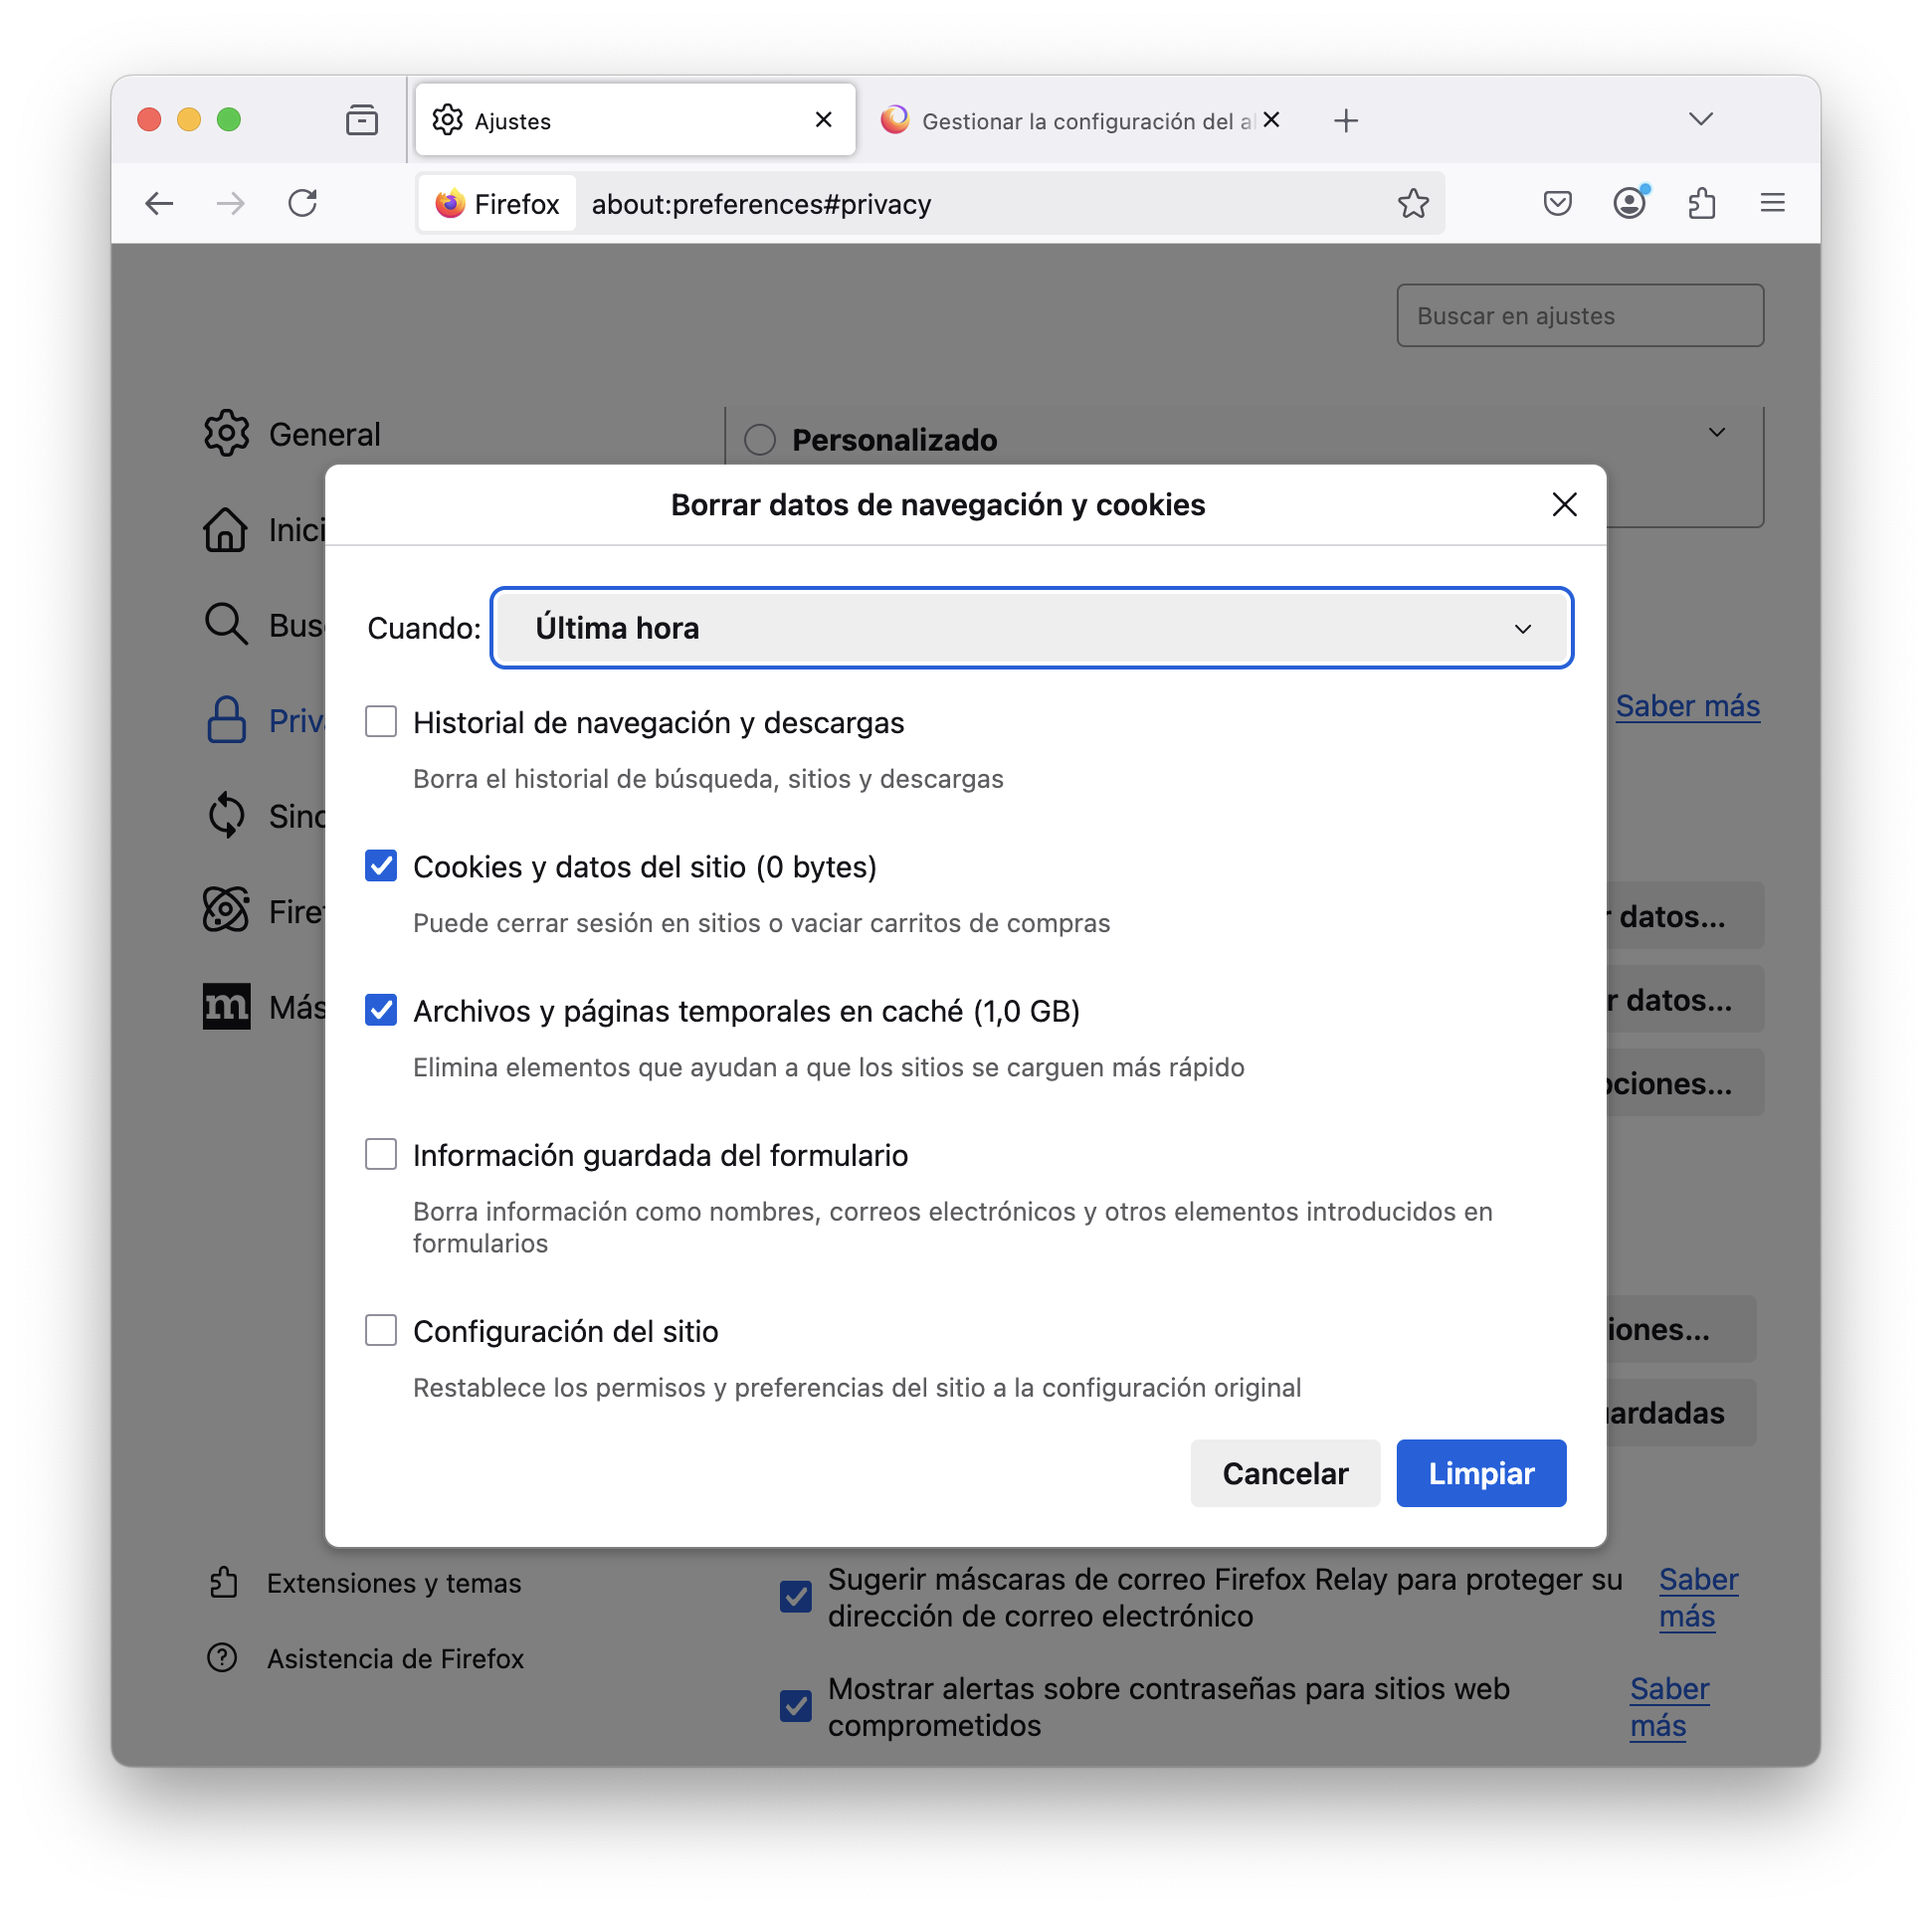
\includegraphics[width=\textwidth]{opcion3_ej14.png}
    \caption{Opción 3 de configuración de cookies, Firefox}
    \label{fig:opcion3_ej14}
\end{figure}

\paragraph{Permitir o bloquear a los sitios que almacenen información }

Esta opción da control al usuario para decidir qué sitios pueden guardar cookies y datos en su dispositivo. Para poder aprovecharla, una vez estamos en la situación de que se muestra en la \ref{fig: opcion3_ej14}, debemos seleccionar la opción “Gestionar excepciones”. Como se ve en la \ref{fig: opcion4_ej14}, se nos permite escribir la dirección exacta del sitio a permitir o bloquear. 

\begin{figure}[H]   
    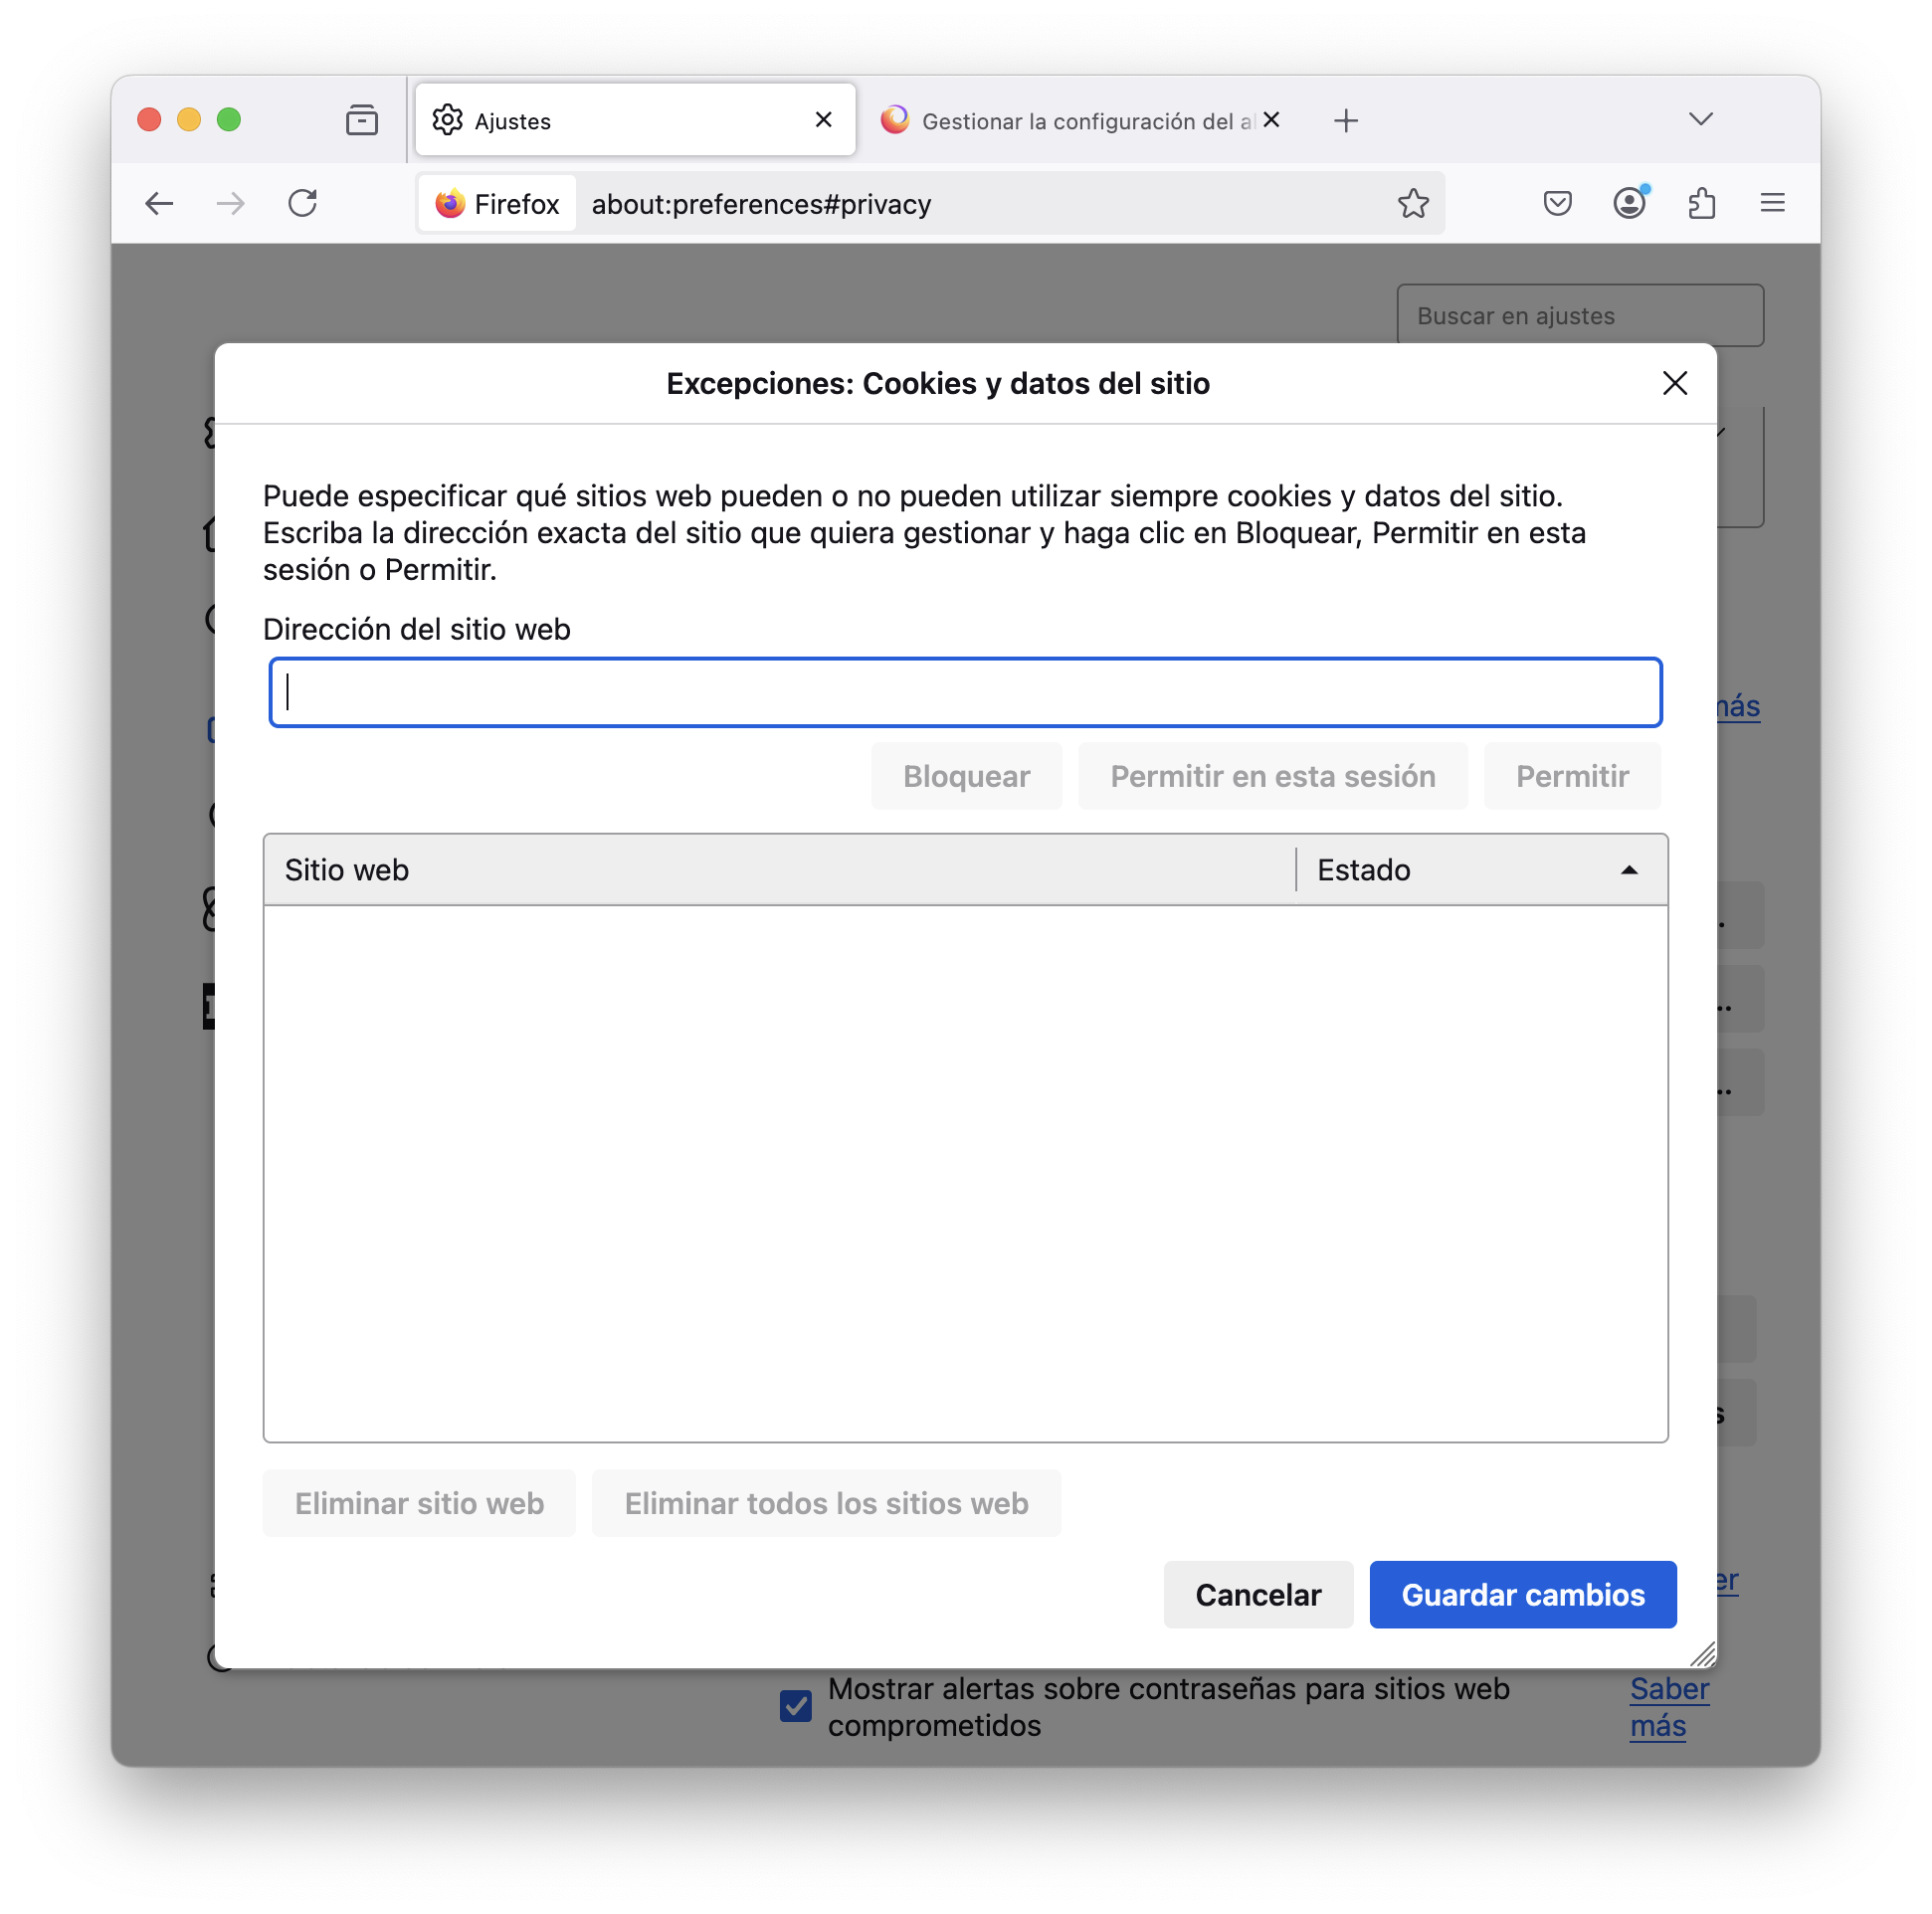
\includegraphics[width=\textwidth]{opcion4_ej14.png}
    \caption{Opción 4 de configuración de cookies, Firefox}
    \label{fig:opcion4_ej14}
\end{figure}


\subsubsection{Configuración cookies Chrome y LibreWolf}

Para poder ver las opciones de gestión de cookies en Google Chrome debemos acceder al menú de configuración y una vez ahí, como se ve en la \ref{fig: cookies_chrome}, podemos acceder a la configuración de "Cookies de terceros". Ahí nos encontramos con tres opciones: 

\paragraph{Permitir cookies de terceros}

Esta opción permite que todos los sitios web usen cookies para seguimiento, personalización o publicidad. 

\paragraph{Bloquear cookies de terceros en modo Incógnito}

Esta opción impide que terceros usen cookies solo cuando se navega en modo incógnito, limitando el rastreo sin afectar la navegación normal. 

\paragraph{Bloquear cookies de terceros}

Esta opción evita completamente que sitios externos a los que se visita usen cookies, aumentando la privacidad pero pudiendo afectar funciones de algunas webs. 

\paragraph{Enviar una solicitud "Do Not Track" con tu tráfico de navegación }

Esta opción solicita a los sitios que no rastreen la actividad del usuario, aunque pueden ignorarlo porque es voluntario. 

\begin{figure}[H]   
    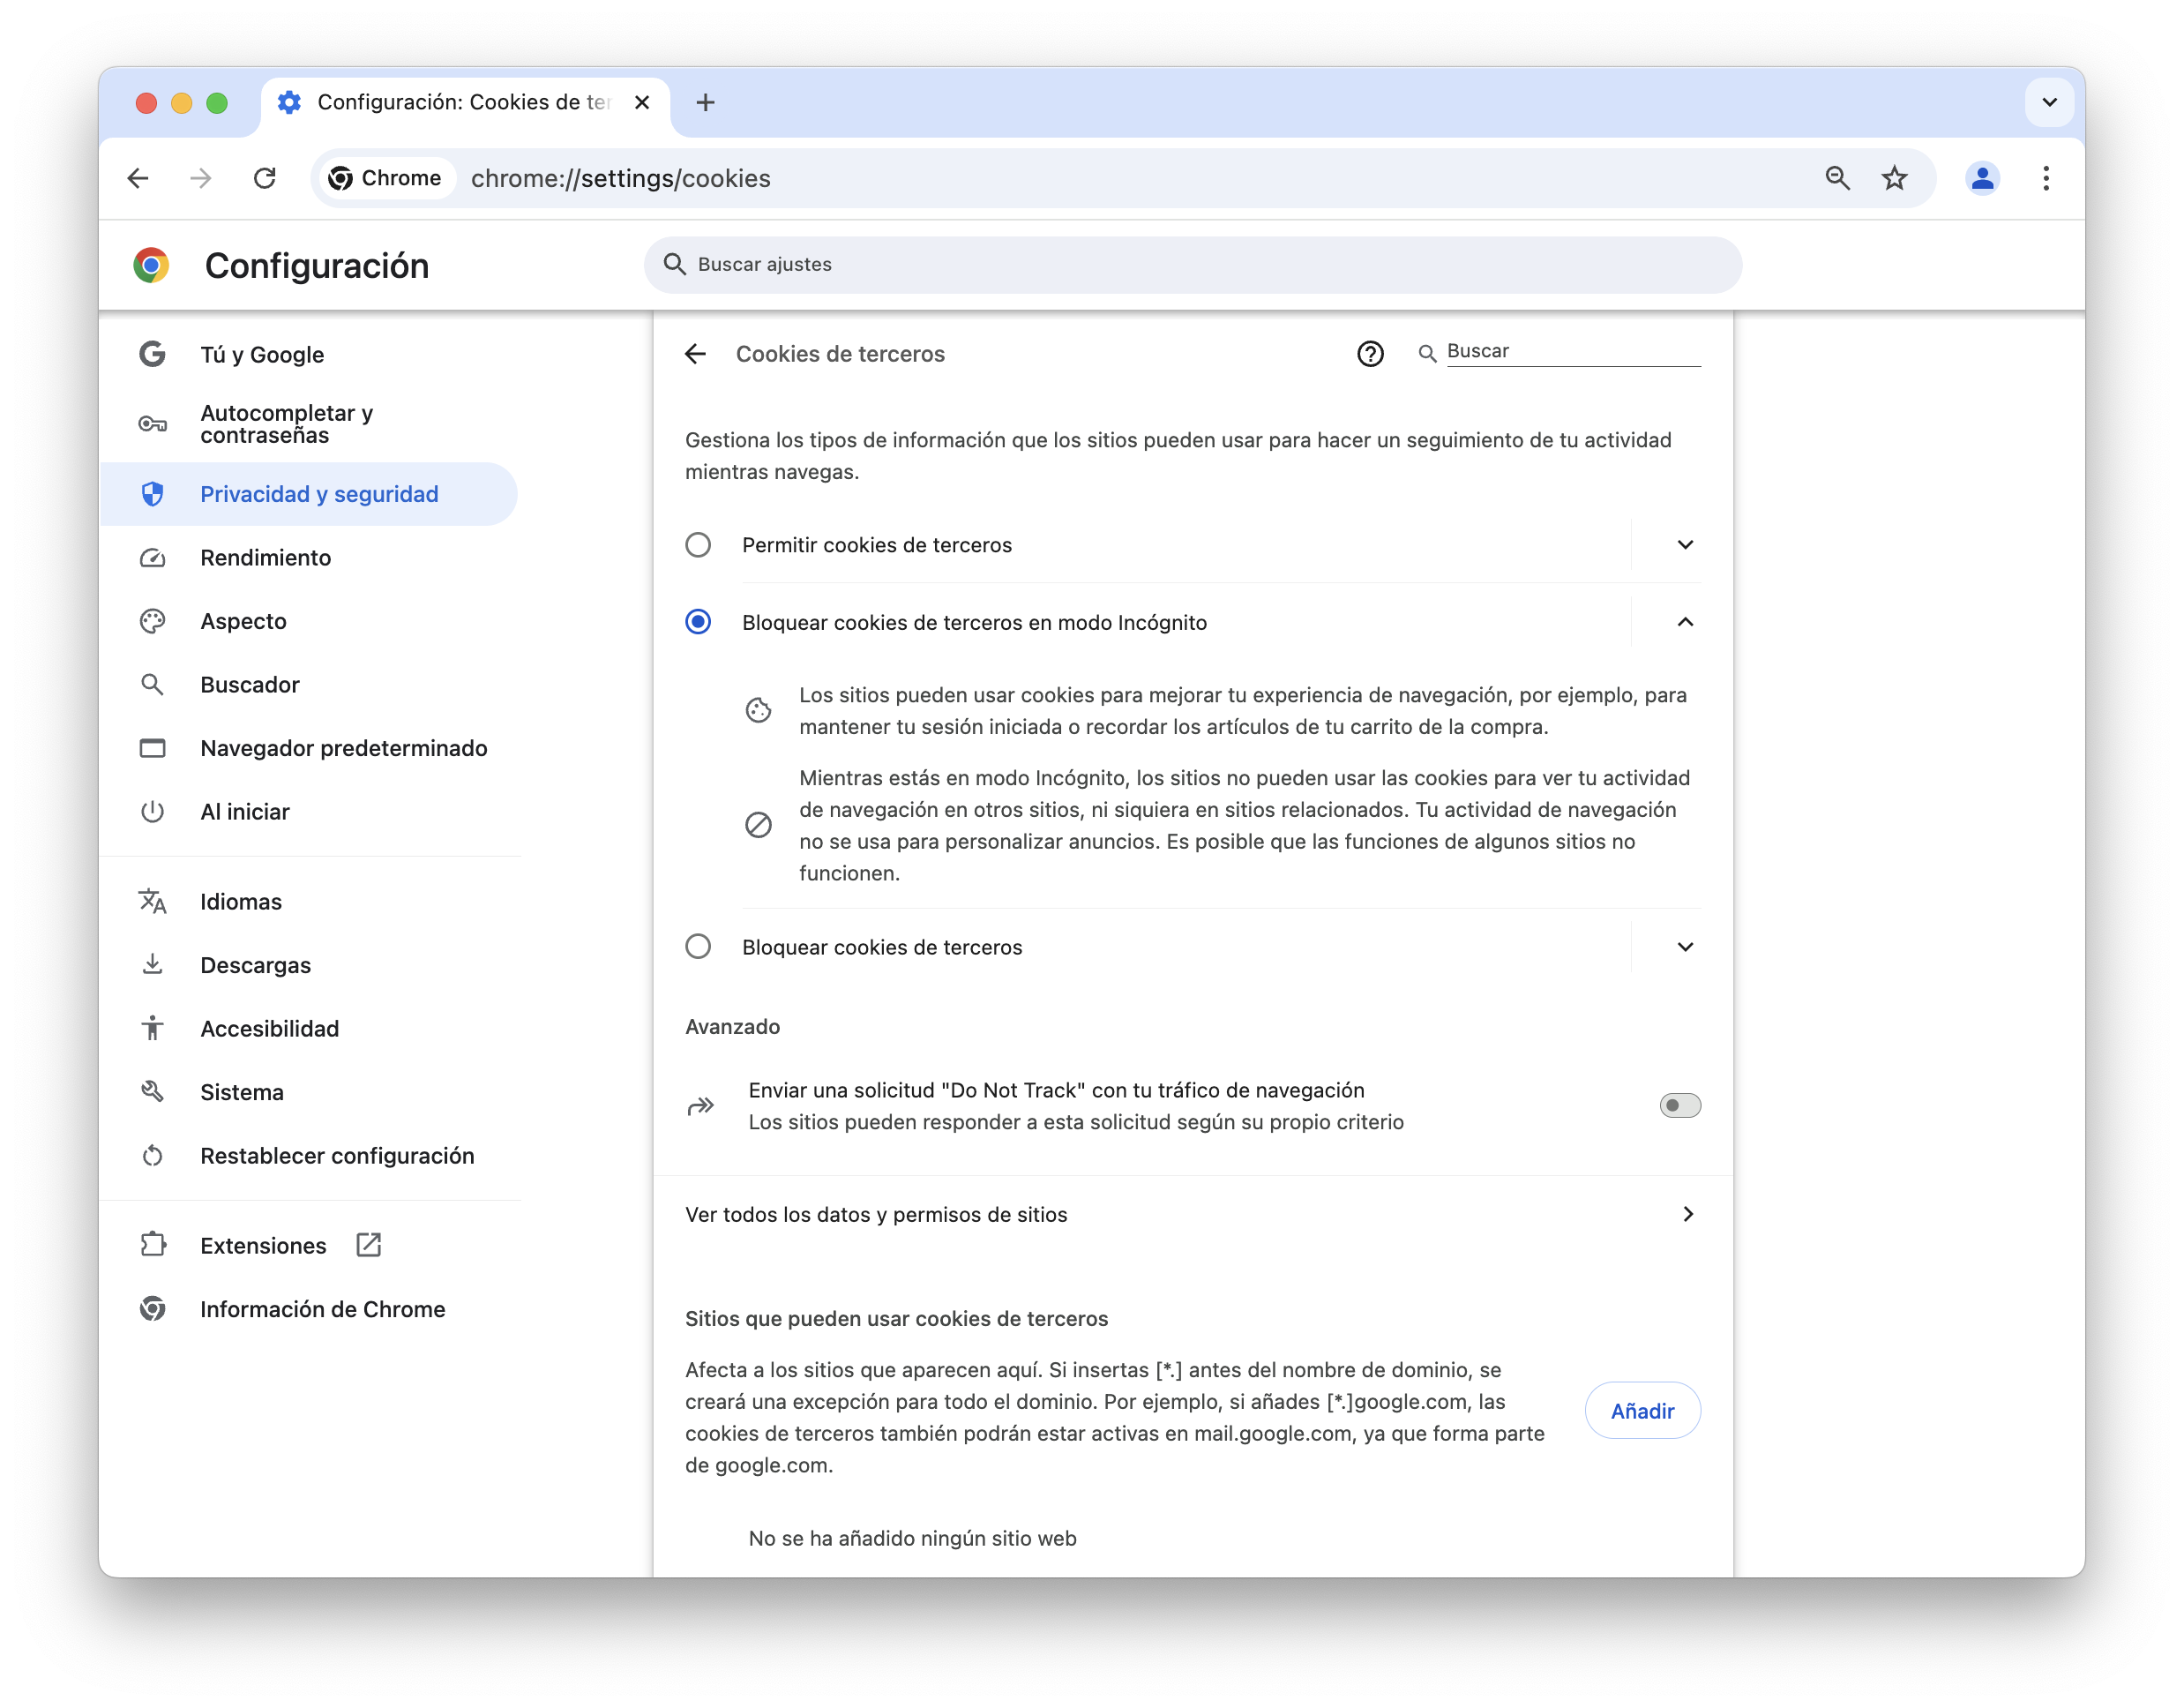
\includegraphics[width=\textwidth]{cookies_chrome_ej14a.png}
    \caption{Configuración de cookies en Chrome}
    \label{fig:cookies_chrome}
\end{figure}

Por otro lado, para acceder a la configuración de cookies de Librewolf, seguimos los pasos anteriores hasta llevar a la \ref{fig: cookies_librewolf}. Como se aprecia, las opciones son aparentemente las mismas que en Mozilla Firefox, explicadas en el apartado anterior. Esto se debe a que Firefox y LibreWolf son navegadores basados en el mismo motor, pero con enfoques diferentes en cuanto a privacidad y control del usuario. Mientras que Firefox ofrece un equilibrio entre personalización, compatibilidad y privacidad, LibreWolf está diseñado específicamente para proteger al máximo la privacidad desde el primer uso. LibreWolf desactiva por defecto toda la telemetría, bloquea rastreadores y cookies de terceros, elimina automáticamente los datos al cerrar el navegador y no incluye integración con servicios de Mozilla. En cambio, Firefox requiere que el usuario configure manualmente muchas de estas opciones para alcanzar el mismo nivel de privacidad. 

\begin{figure}[H]   
    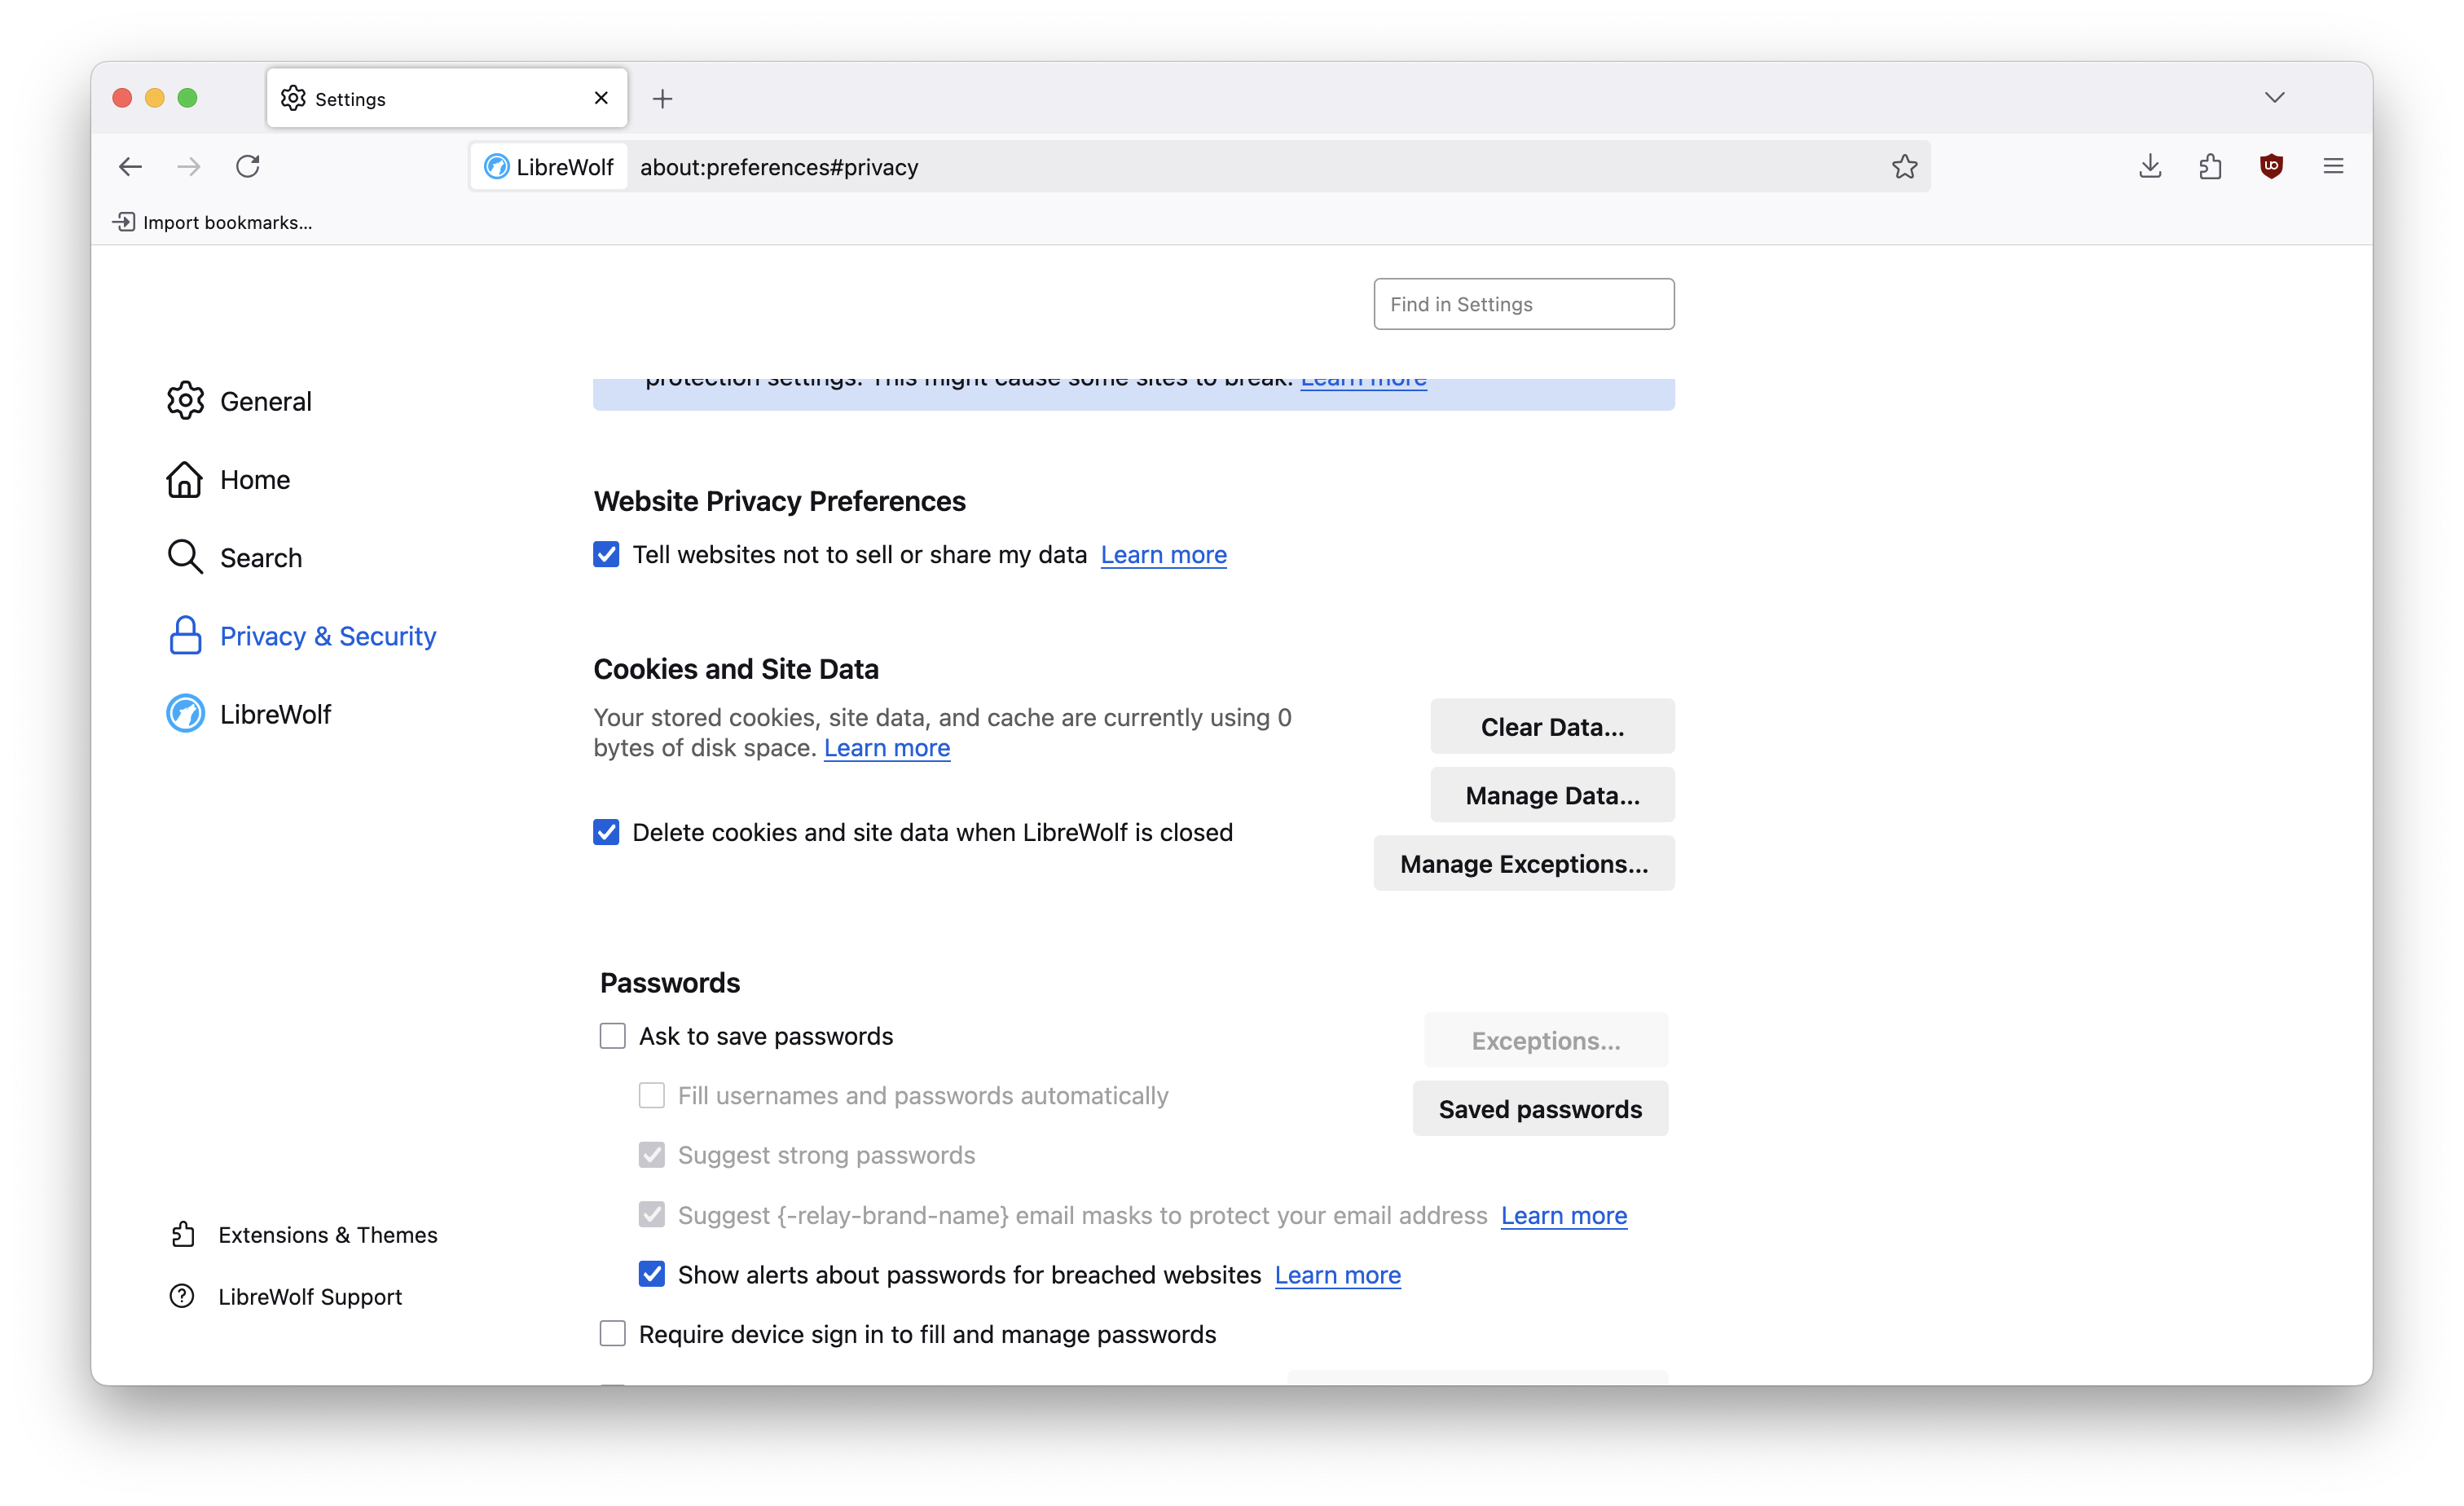
\includegraphics[width=\textwidth]{cookies_librewolf_ej14a.png}
    \caption{Configuración de cookies en LibreWolf}
    \label{fig:cookies_librewolf}
\end{figure}

En \ref{comparativa-cookies} podemos ver una comparación más visual de los 3 buscadores.

\begin{table}[H]
    \centering
    \begin{tabular}{|l|c|c|c|}
    \hline
    \textbf{Característica} & \textbf{Firefox} & \textbf{LibreWolf} & \textbf{Chrome} \\ \hline
    Permitir todas las cookies & Sí (manual) & No (privacidad estricta) & Sí (por defecto) \\ \hline
    Bloquear cookies de terceros & Sí (opción manual) & Sí (activado por defecto) & Sí (opción disponible) \\ \hline
    Eliminar cookies al cerrar & Opcional & Activado por defecto & Opcional \\ \hline
    Telemetría y rastreo & Activado (puede desactivarse) & Desactivado & Activado (puede limitarse) \\ \hline
    Protección de privacidad & Alta (manual) & Muy alta (por defecto) & Media (requiere configurarlo) \\ \hline
    \end{tabular}
    \caption{Comparativa de opciones de configuración de cookies en Firefox, LibreWolf y Chrome.}
    \label{tab:comparativa-cookies}
\end{table}

\subsubsection{Extensiones de navegador para la gestión de cookies}

\paragraph{Cookie AutoDelete}

Cookie AutoDelete es una extensión de navegador diseñada para gestionar automáticamente las cookies y otros datos de sitios web. Su principal función es eliminar las cookies asociadas a una pestaña en cuanto esta se cierra, evitando que los sitios web rastreen al usuario en futuras visitas. Además, permite crear listas blancas (whitelists) para conservar las cookies de sitios de confianza y listas grises (greylists) para eliminar cookies al reiniciar el navegador. La extensión también ofrece opciones para eliminar manualmente cookies y otros datos de almacenamiento, como IndexedDB y LocalStorage, y es compatible con las pestañas de contenedor en Firefox [\url{cookie_autodelete.gal}]

\paragraph{Privacy Badger}

Privacy Badger, desarrollado por la Electronic Frontier Foundation (EFF), es una extensión de navegador que bloquea automáticamente rastreadores invisibles y cookies de terceros sin necesidad de configuración previa. A diferencia de los bloqueadores tradicionales basados en listas predefinidas, Privacy Badger utiliza un algoritmo de aprendizaje automático que detecta y bloquea dominios en función de su comportamiento de rastreo a lo largo de los sitios web visitados. Además, Privacy Badger envía señales como "Do Not Track" y "Global Privacy Control" para solicitar a los sitios web que no rastreen ni vendan la información del usuario. Si un dominio ignora estas señales y sigue rastreando, Privacy Badger lo bloquea automáticamente, fortaleciendo la privacidad de la navegación sin necesidad de intervención manual [\url{privacybadger.gal}]. 

\paragraph{Pruebas}

Para probar ambas extensiones del navegador, debemos instalarlas. En nuestro caso, elegimos Firefox como navegador. En las \ref{fig: addon_cookie_autodelete} y \ref{fig:addon_privacybadger} se ven las extensiones a instalar. Tras la instalación, se debe activar la extensión en el navegador de Cookie Autodelete, como se ve en la \ref{fig: activacion_cookie_autodelete}, mientras que Privacy Badger aparece automáticamente en la barra de extensiones. 

El siguiente paso es buscar una página web que utilice cookies. Lo ideal es hacer la prueba con páginas grandes que suelan tener rastreadores, como medios de comunicación o redes sociales. En nuestro caso, elegimos la página web del periódico La Voz de Galicia.  

Como se ve en \ref{fig:cookies_lavoz}, al entrar en la página nos aparece una pestaña para gestionar las cookies. Para comprobar el funcionamiento de las extensiones, debemos aceptar las cookies del sitio. Inmediatamente, aparecerán notificaciones de ambas extensiones, indicando que se han detectado correctamente los rastreadores y cookies. En \ref{fig:resultado_cookies_autodelete} y \ref{fig:resultado_privacybadger} vemos los resultados. Destacamos que Privacy Badger señala de color verde a los rastreadores que permite, de amarillo a los rastreadores que permite parcialmente, y de rojo a los bloqueados. 

\begin{figure}[H]   
    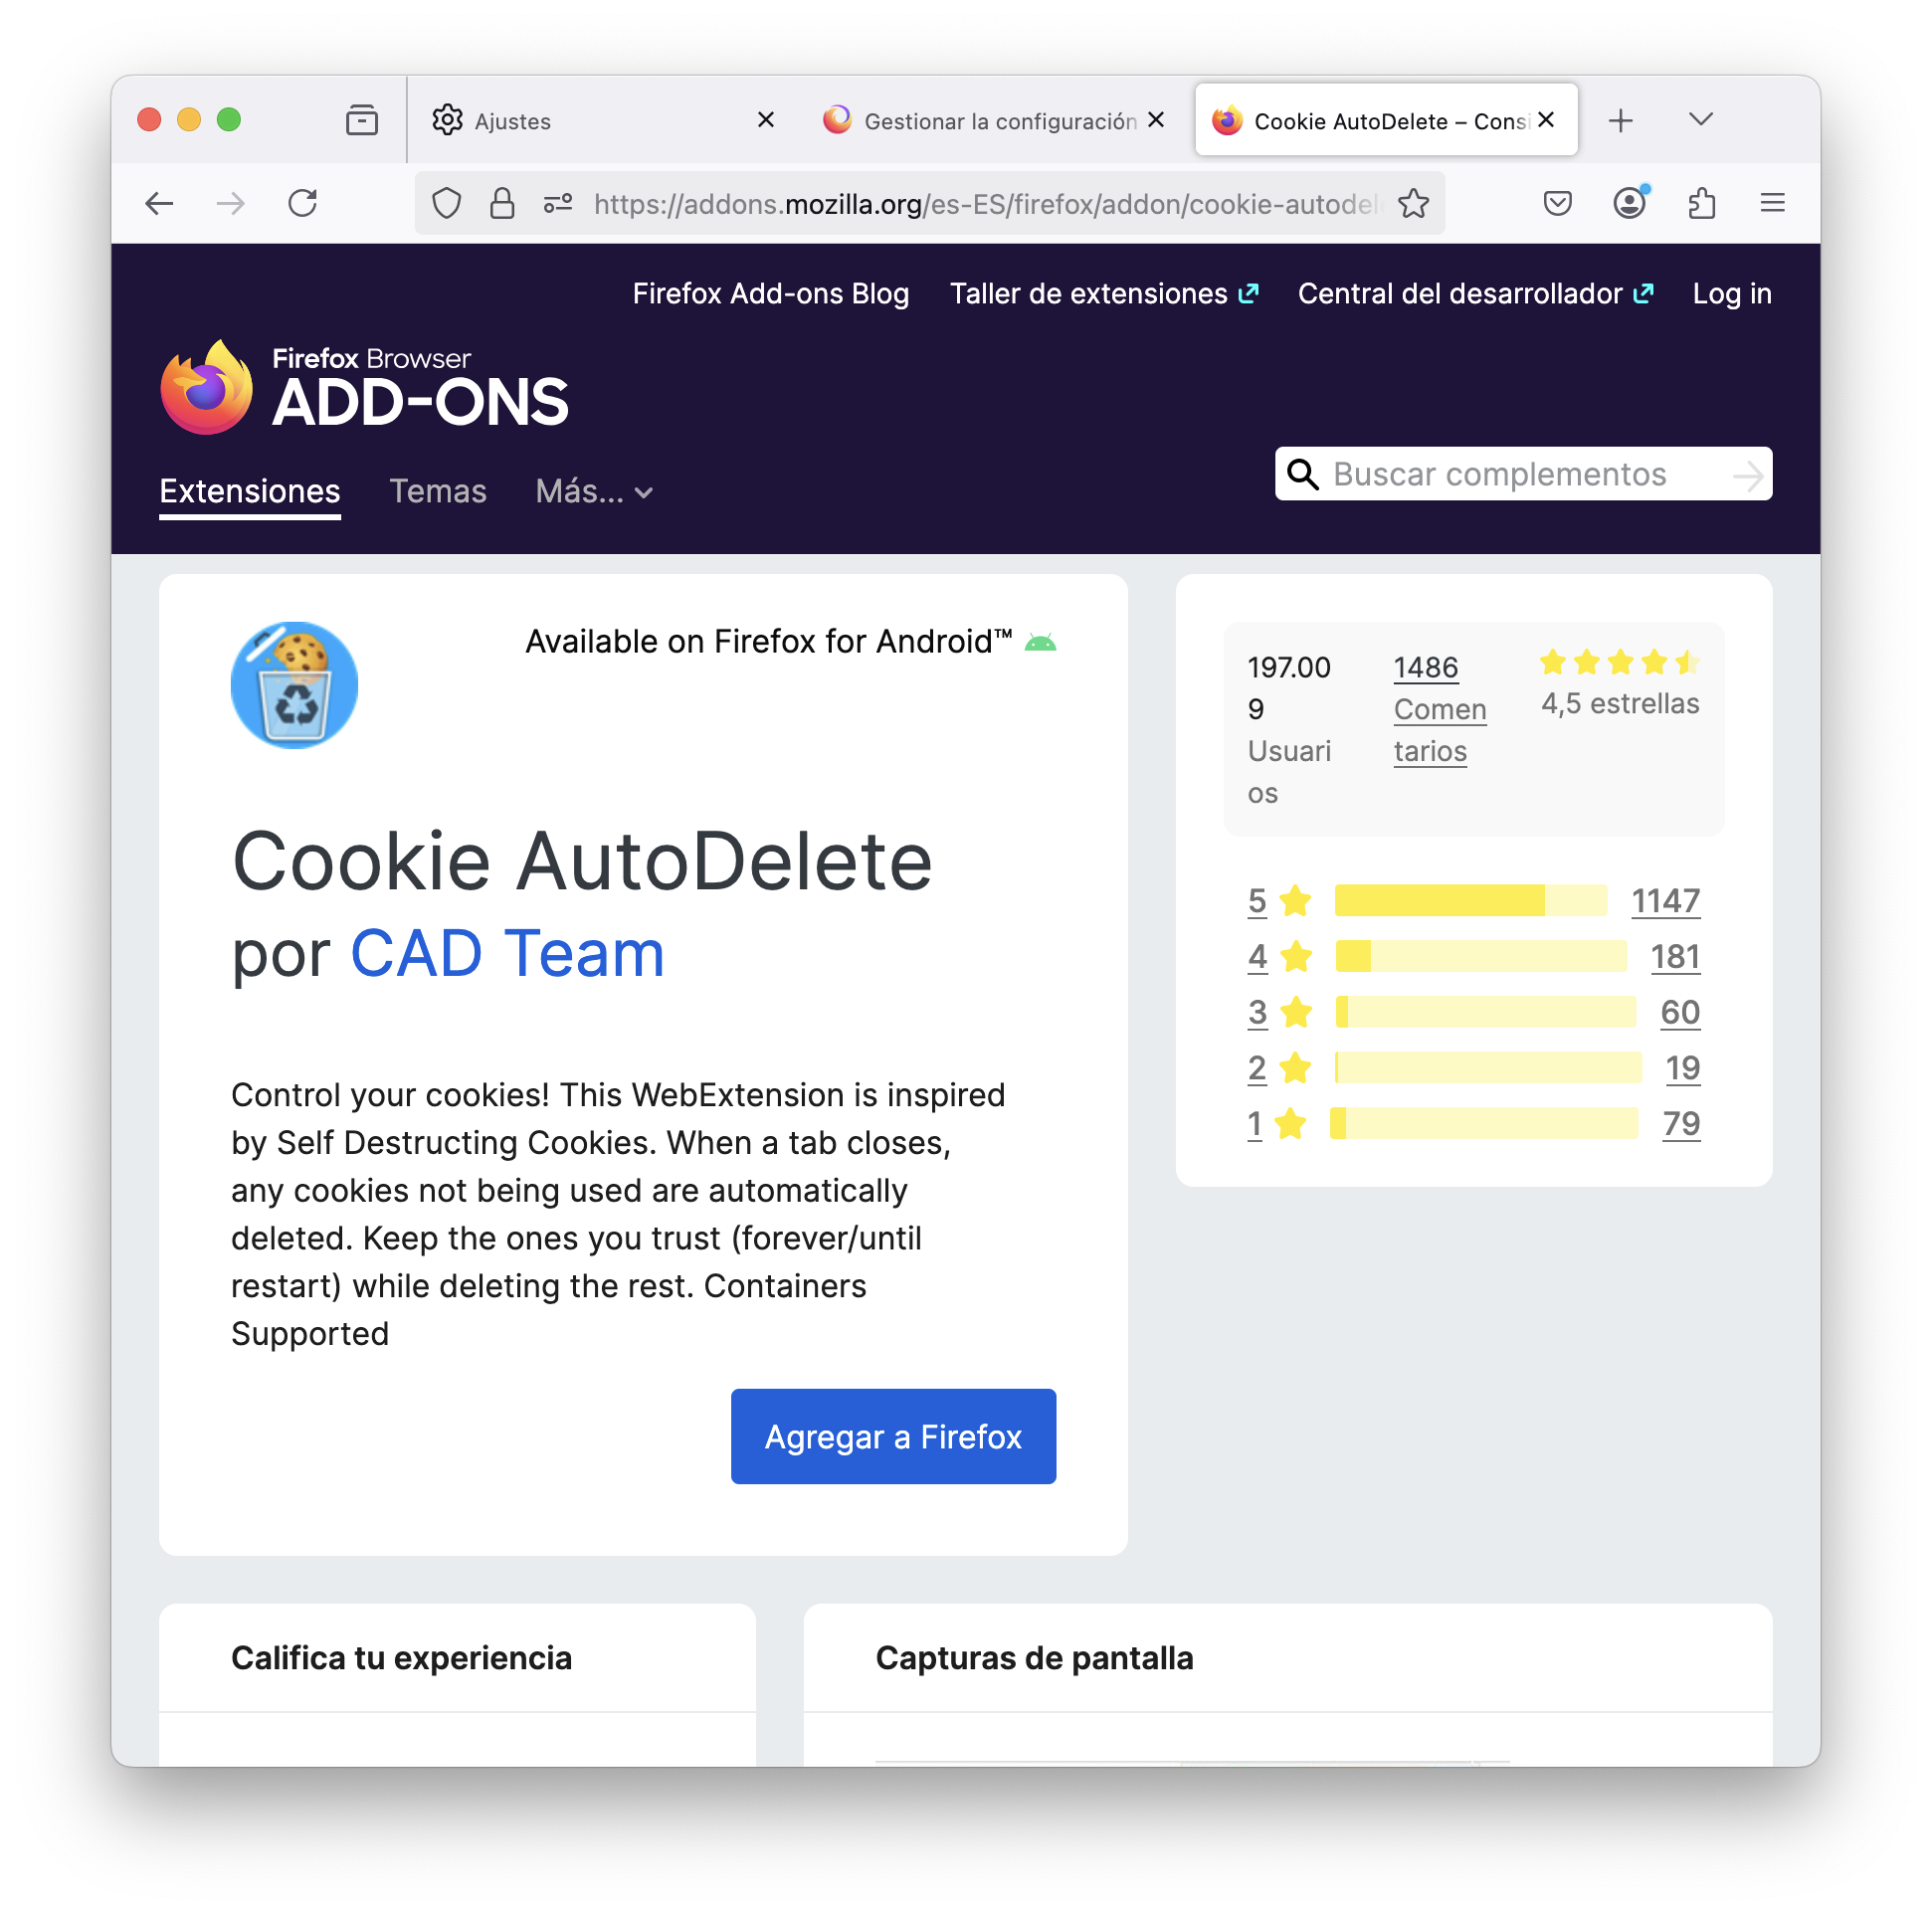
\includegraphics[width=\textwidth]{addon_cookie_autodelete.png}
    \caption{Add on de cookie Autodelete}
    \label{fig:addon_cookie_autodelete}
\end{figure}

\begin{figure}[H]   
    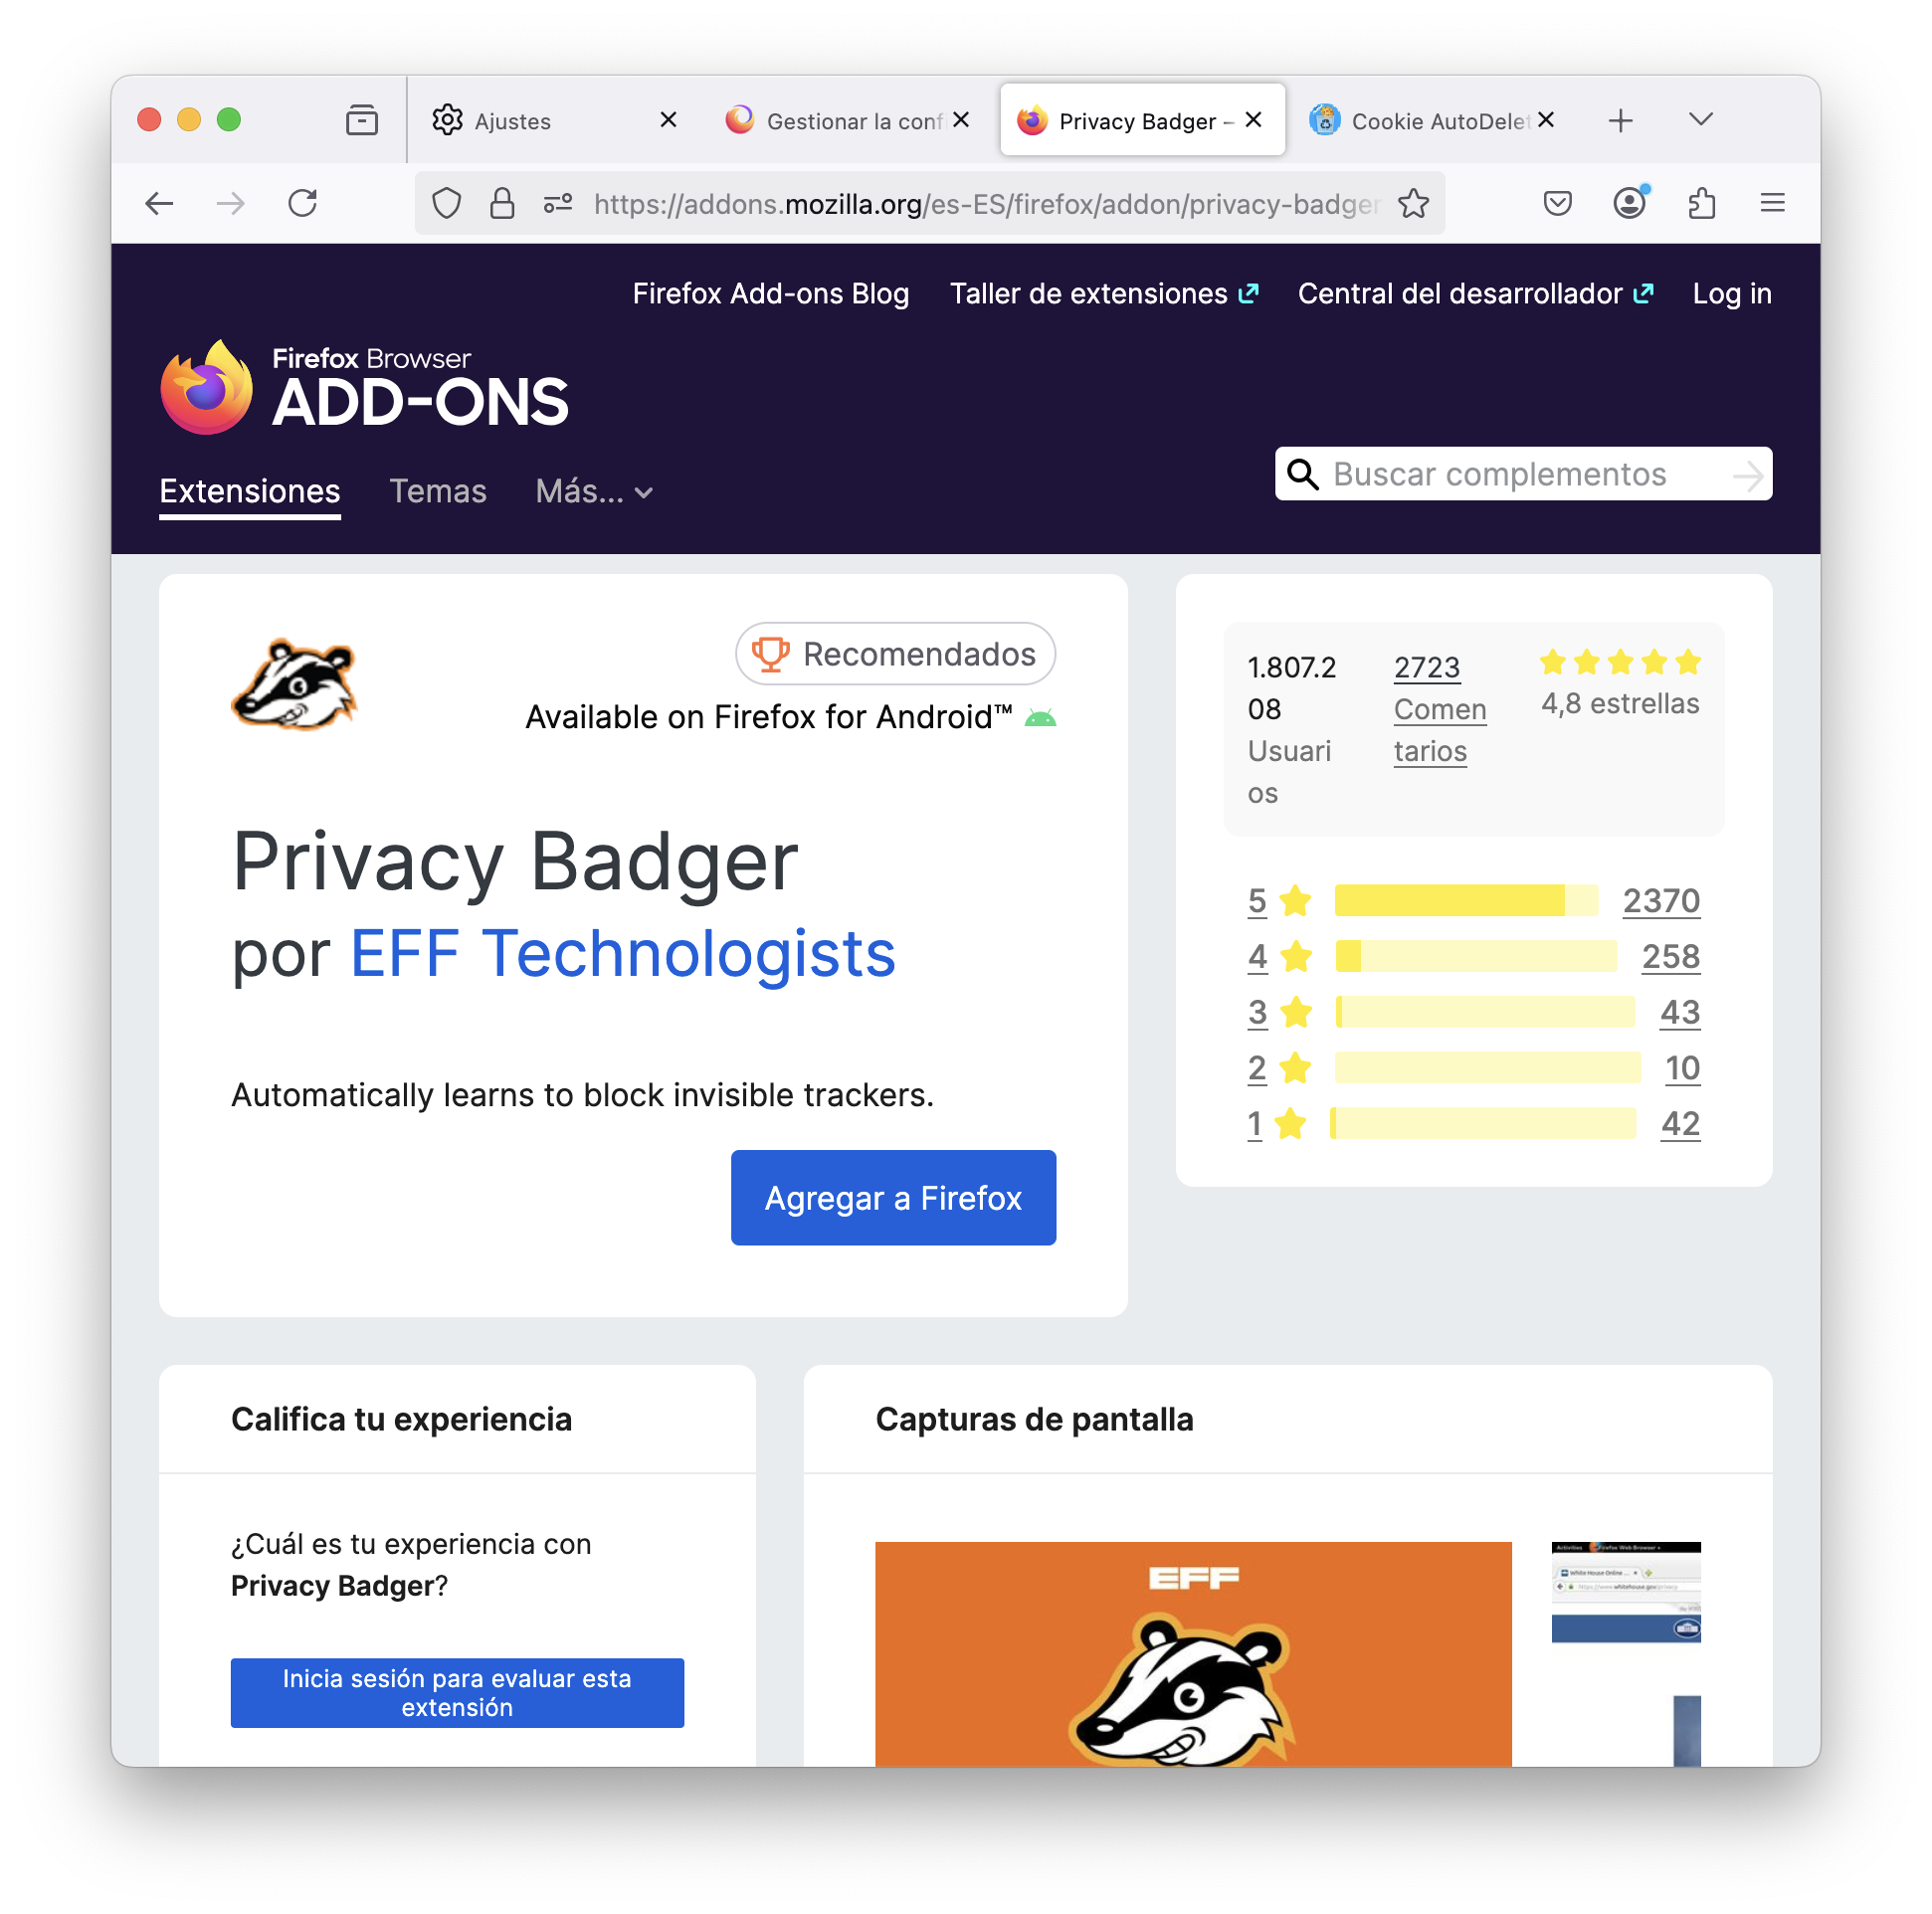
\includegraphics[width=\textwidth]{addon_privacybadger.png}
    \caption{Add on de Privacy Badger}
    \label{fig:addon_privacybadger}
\end{figure}

\begin{figure}[H]   
    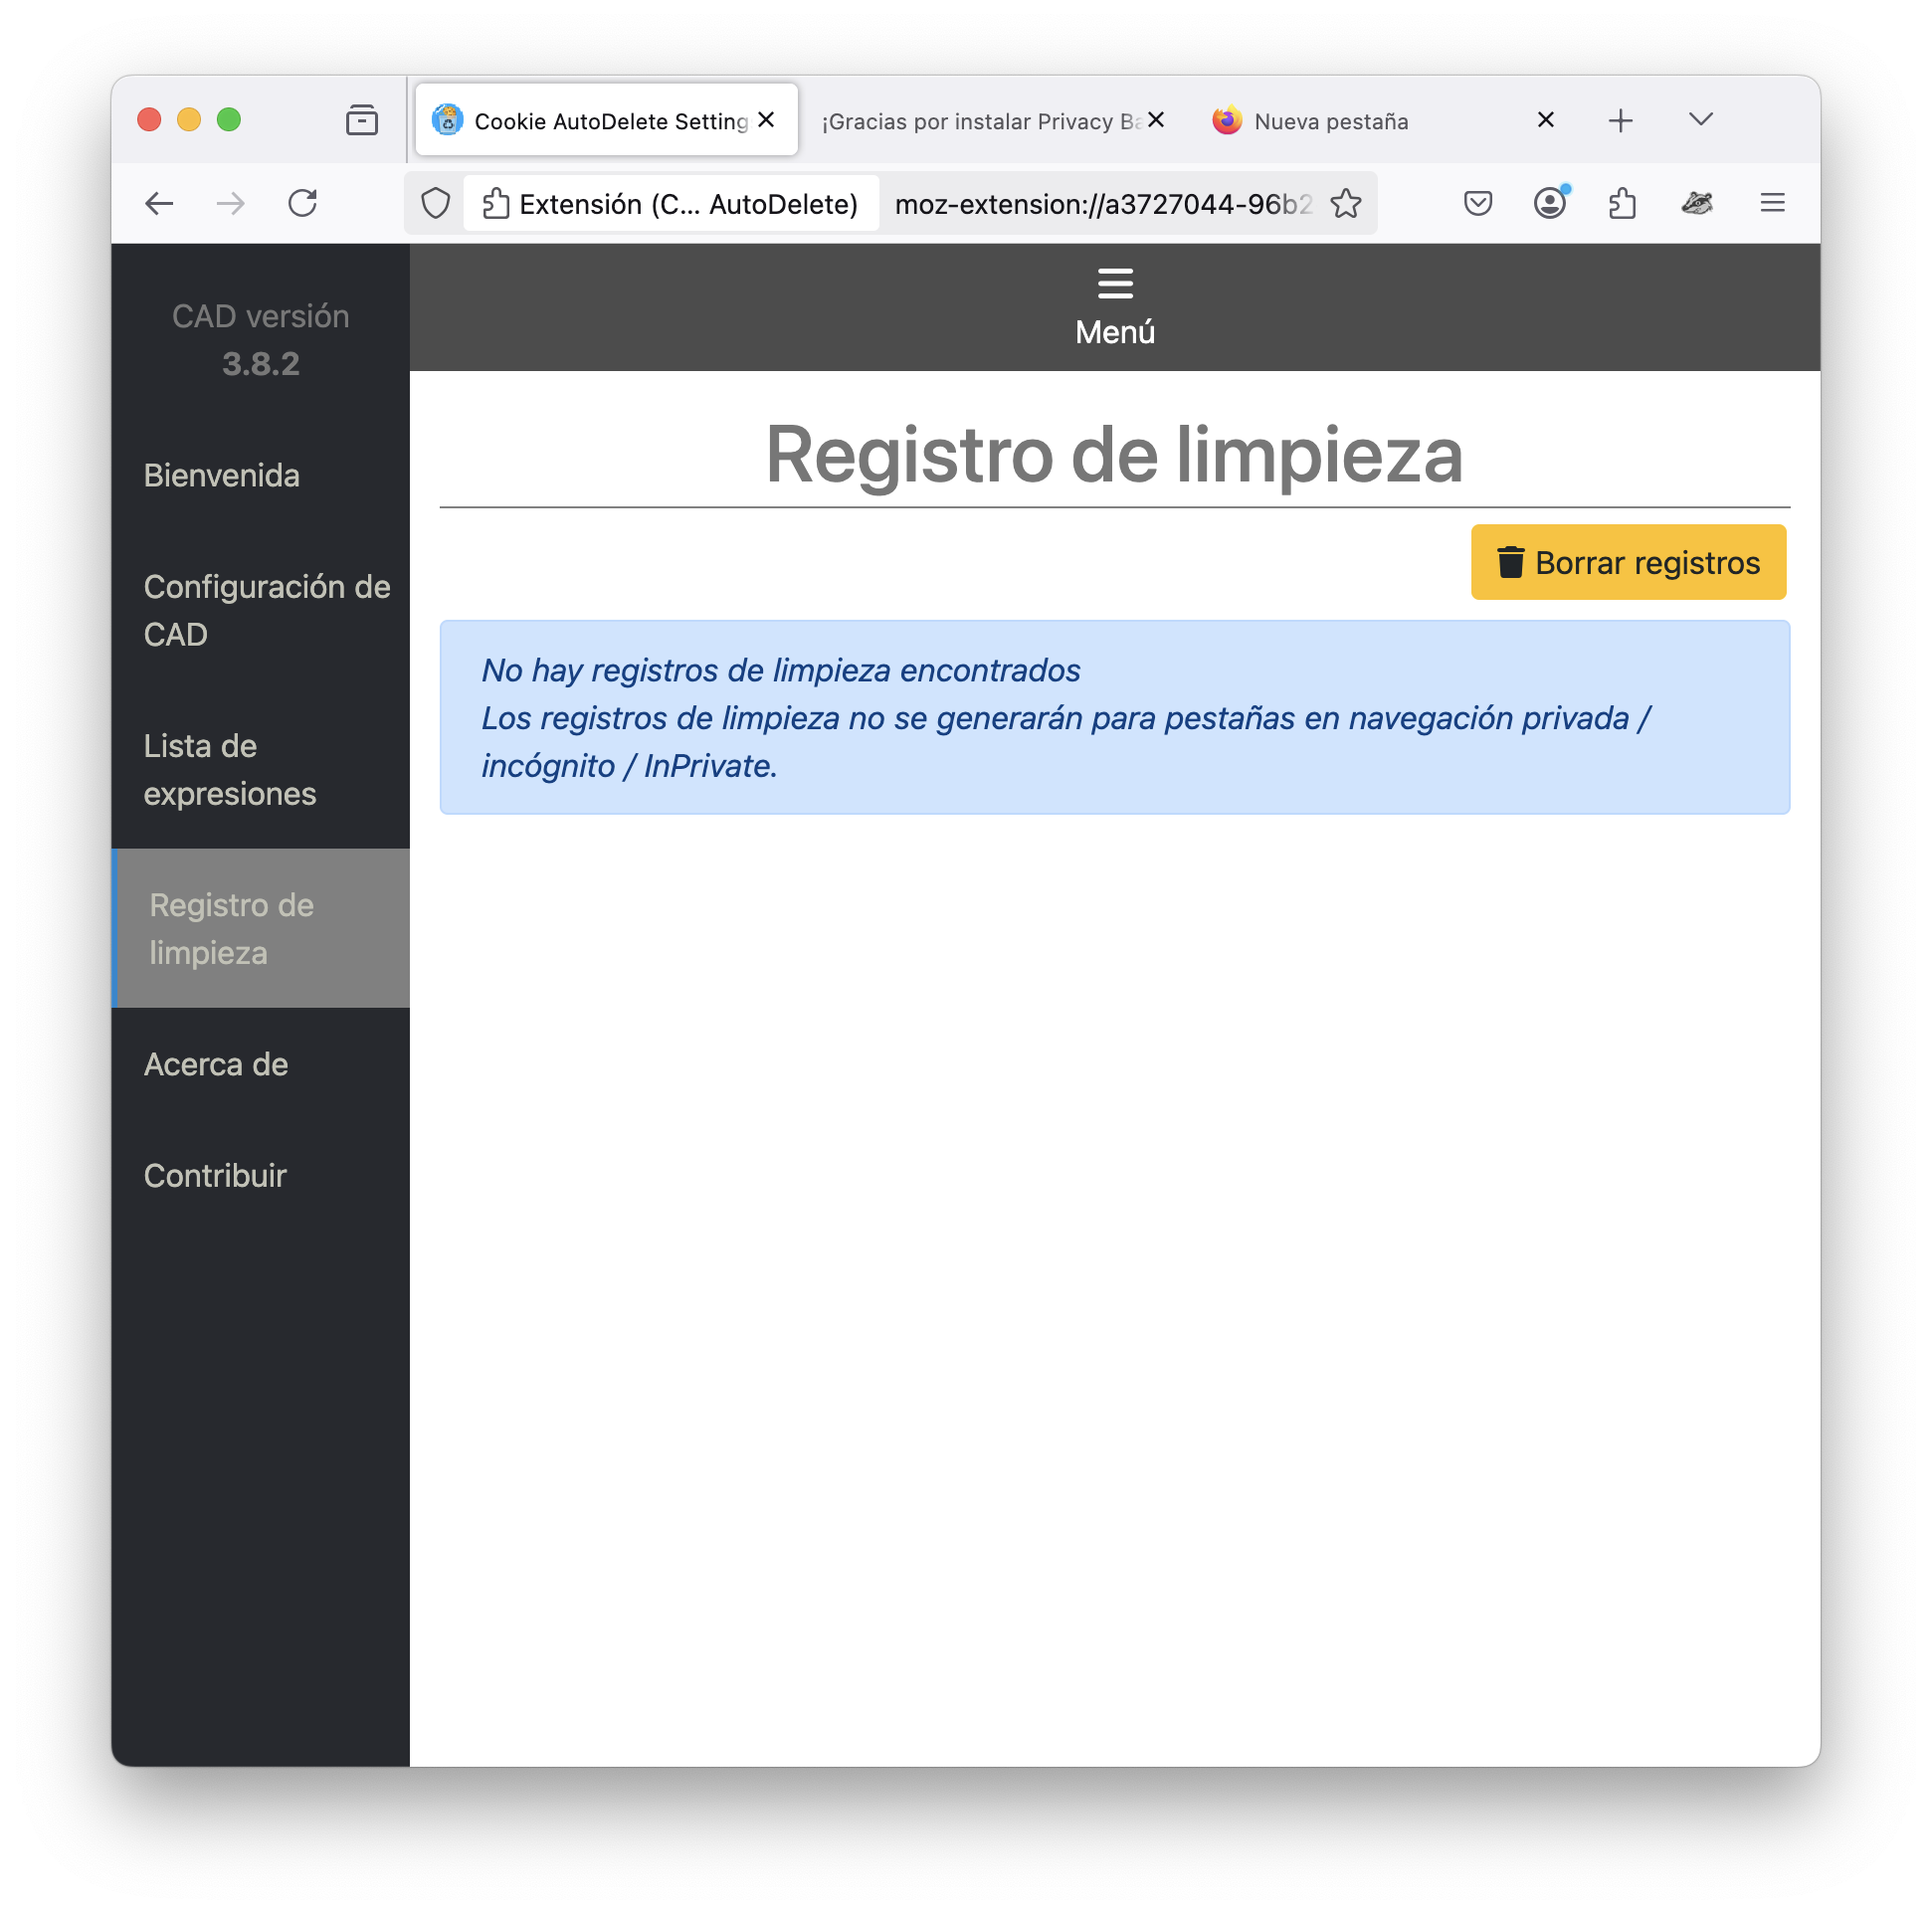
\includegraphics[width=\textwidth]{activacion_cookie_autodelete.png}
    \caption{Activacion Cookie Autodelete}
    \label{fig:activacion_cookie_autodelete}
\end{figure}

\begin{figure}[H]   
    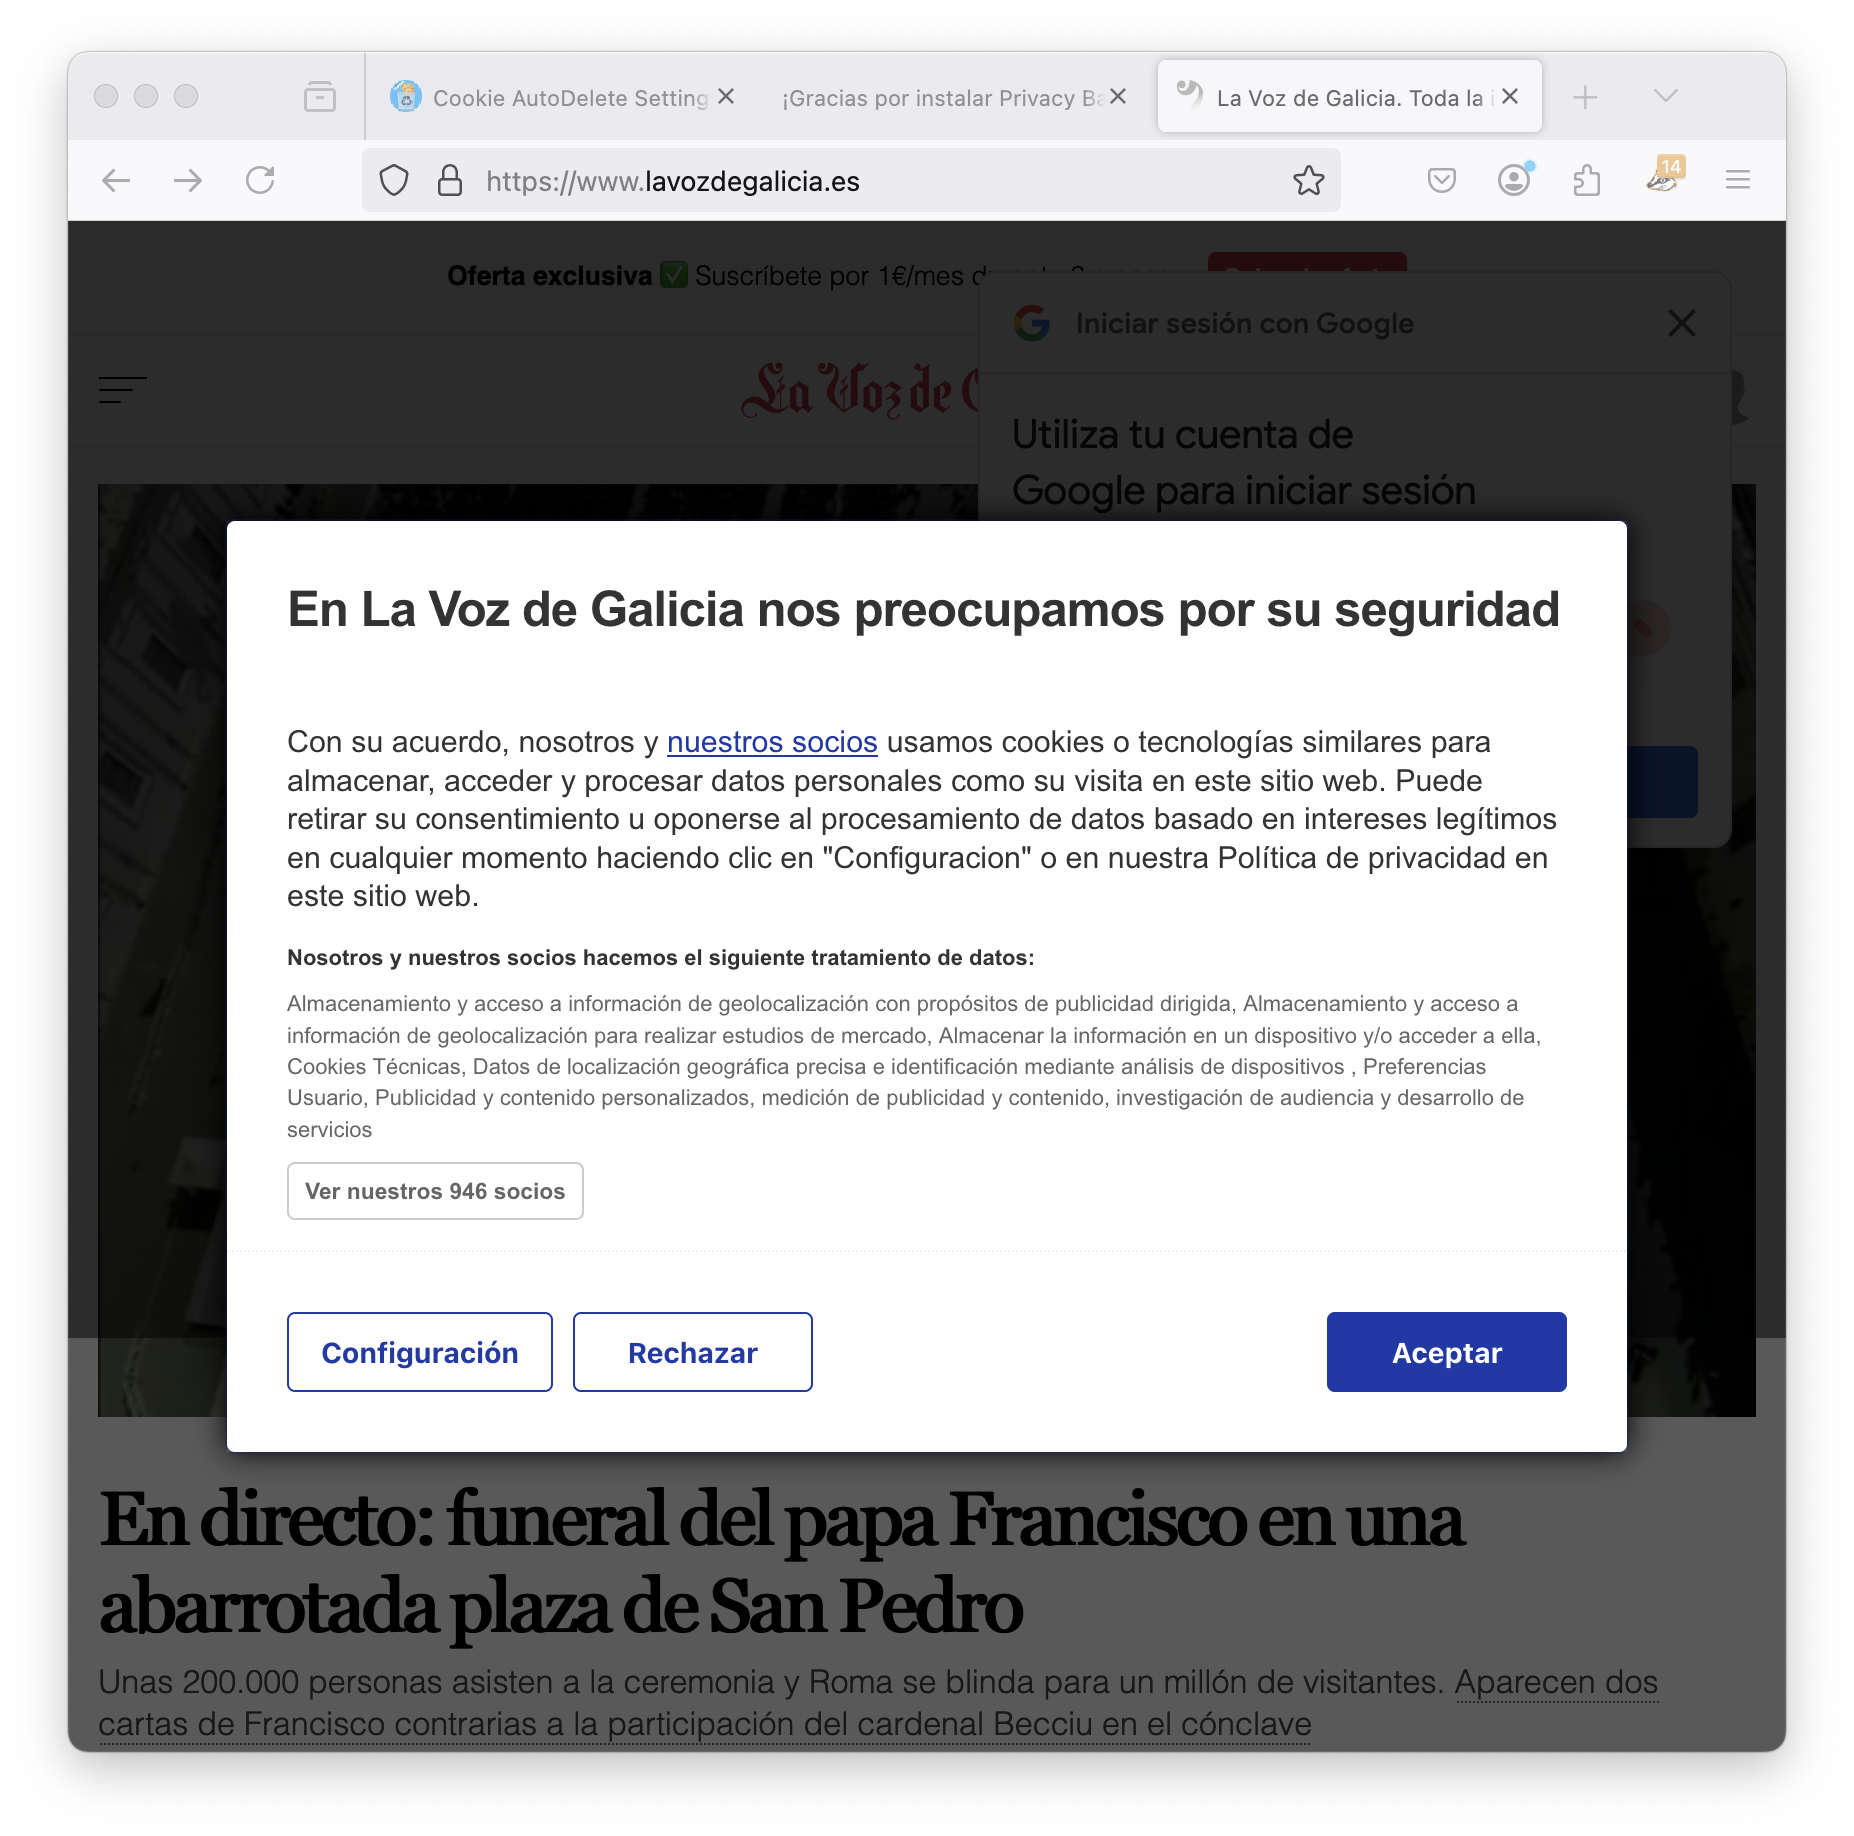
\includegraphics[width=\textwidth]{cookies_lavoz.png}
    \caption{Cookies la Voz de Galicia}
    \label{fig:cookies_lavoz}
\end{figure}

\begin{figure}[H]   
    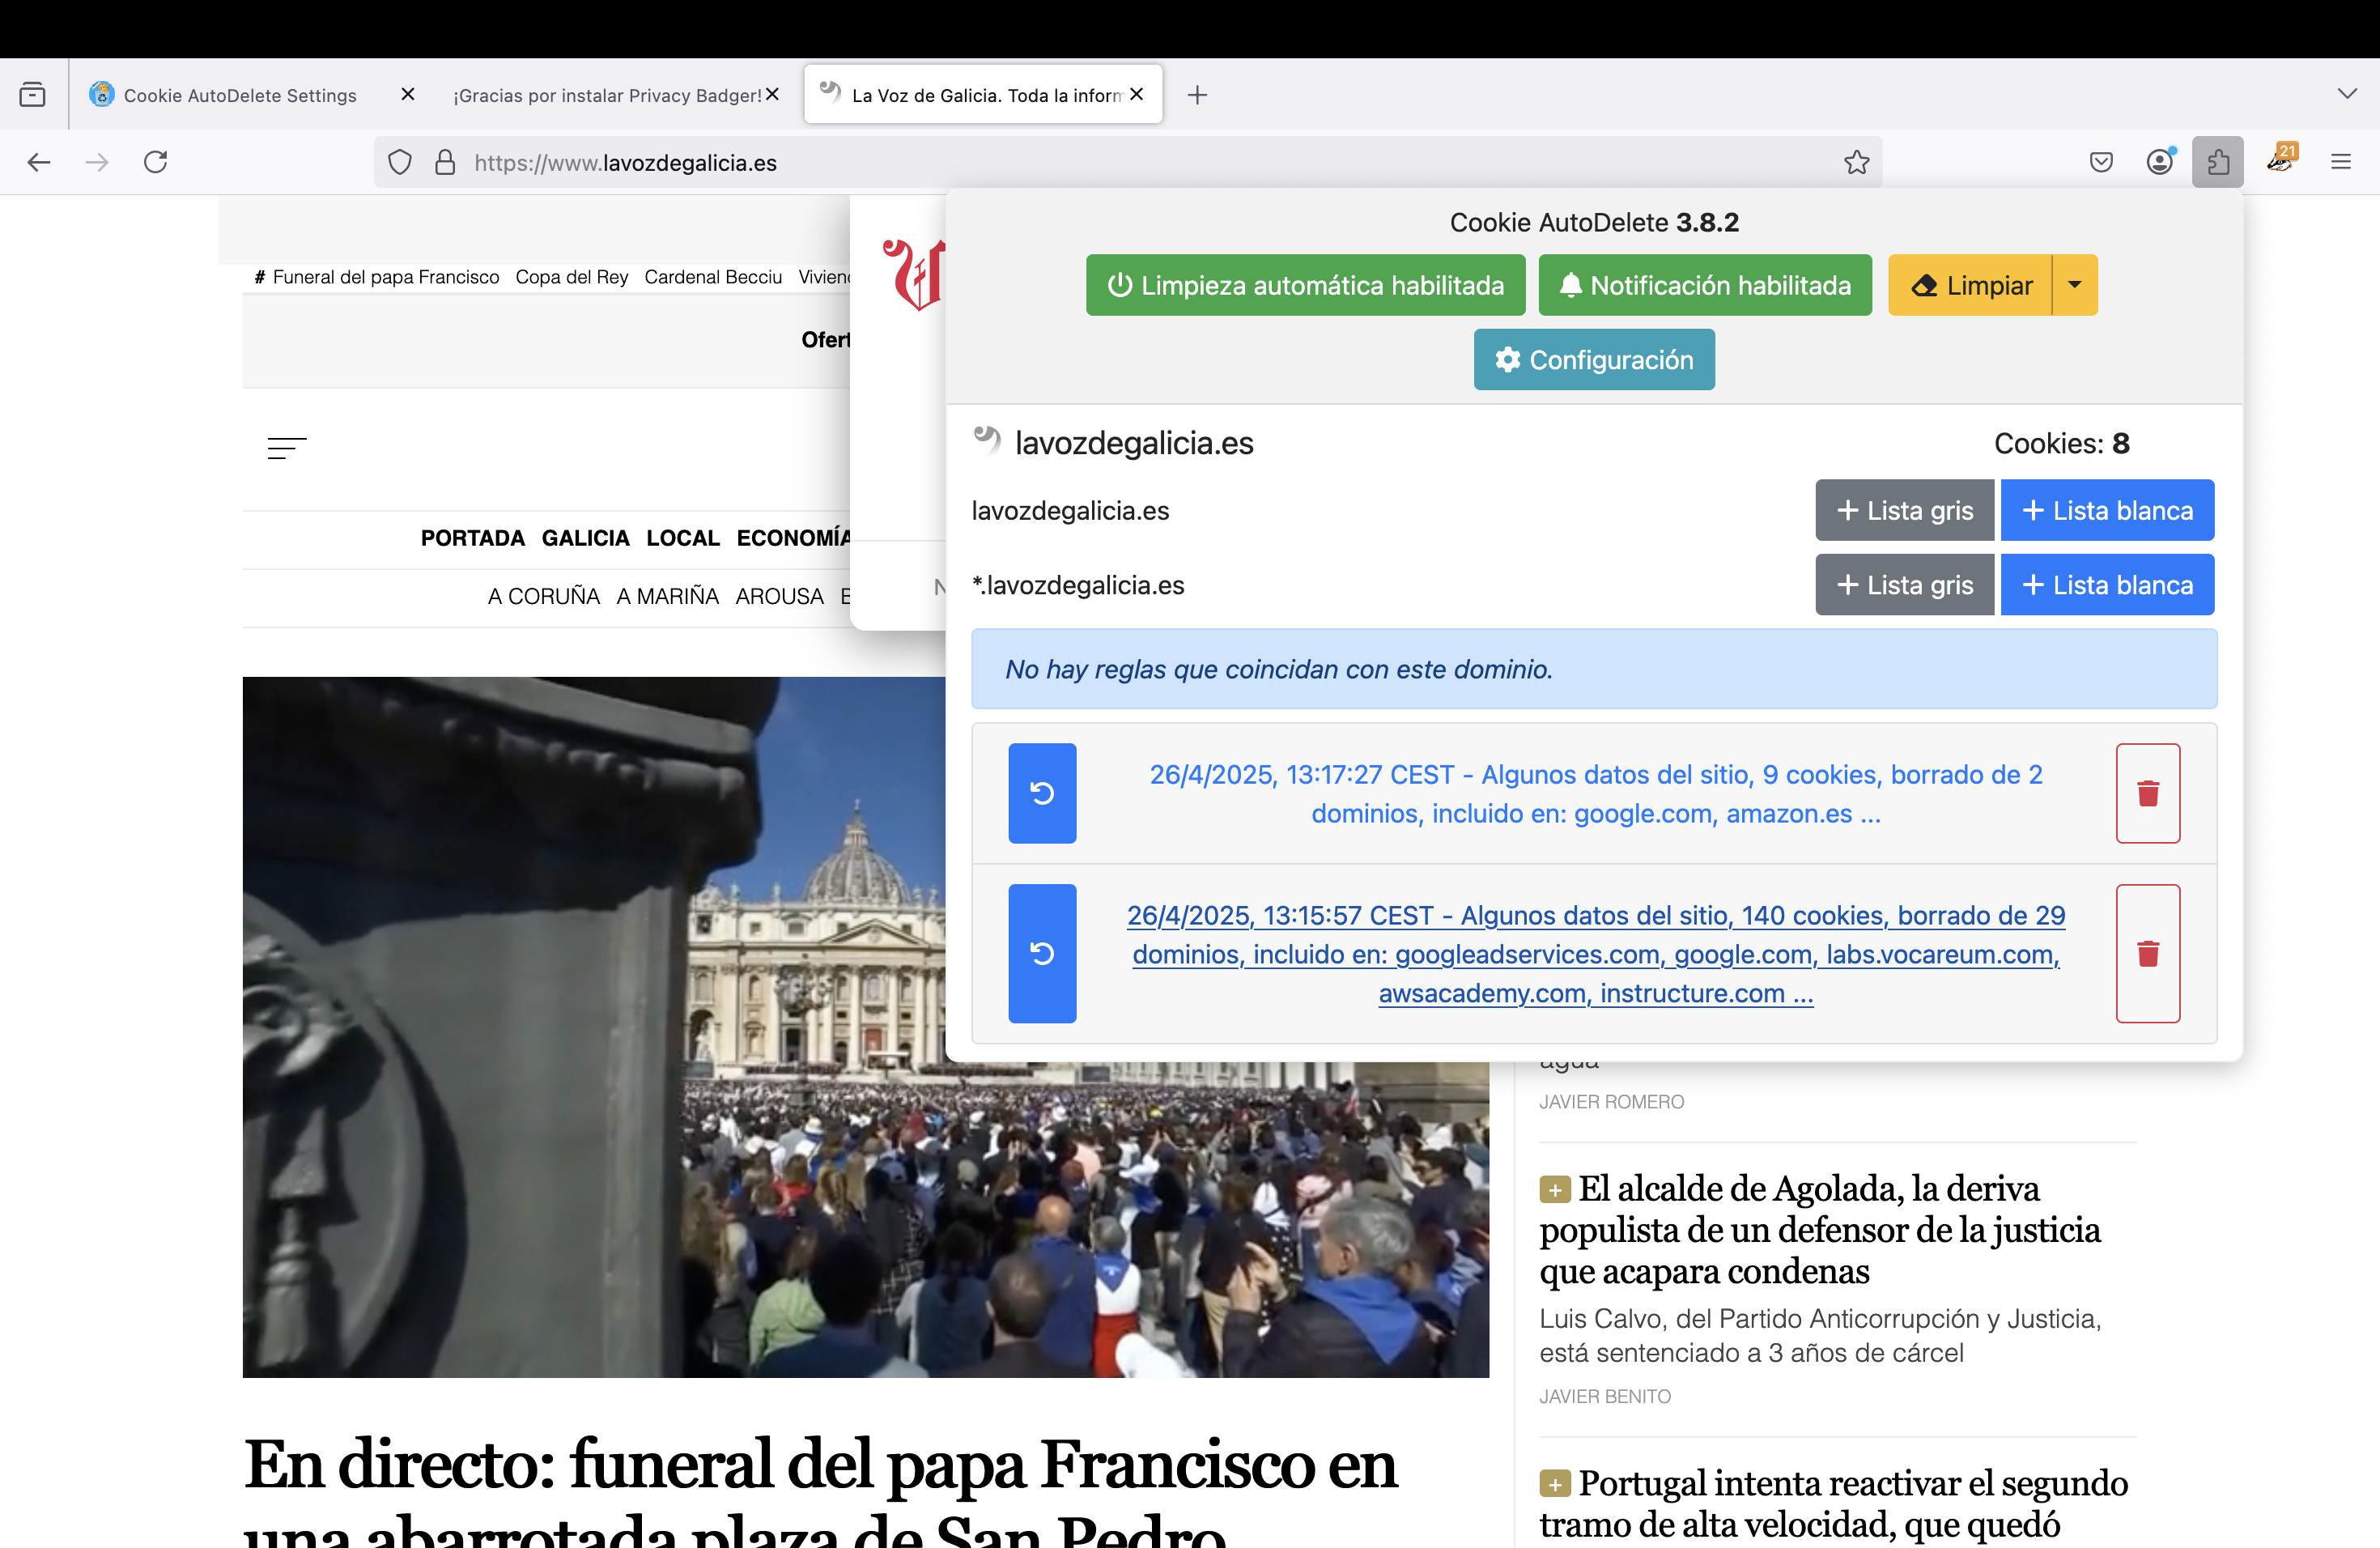
\includegraphics[width=\textwidth]{resultado_cookies_autodelete.png}
    \caption{Resultado Cookies Autodelete}
    \label{fig:resultado_cookies_autodelete}
\end{figure}

\begin{figure}[H]   
    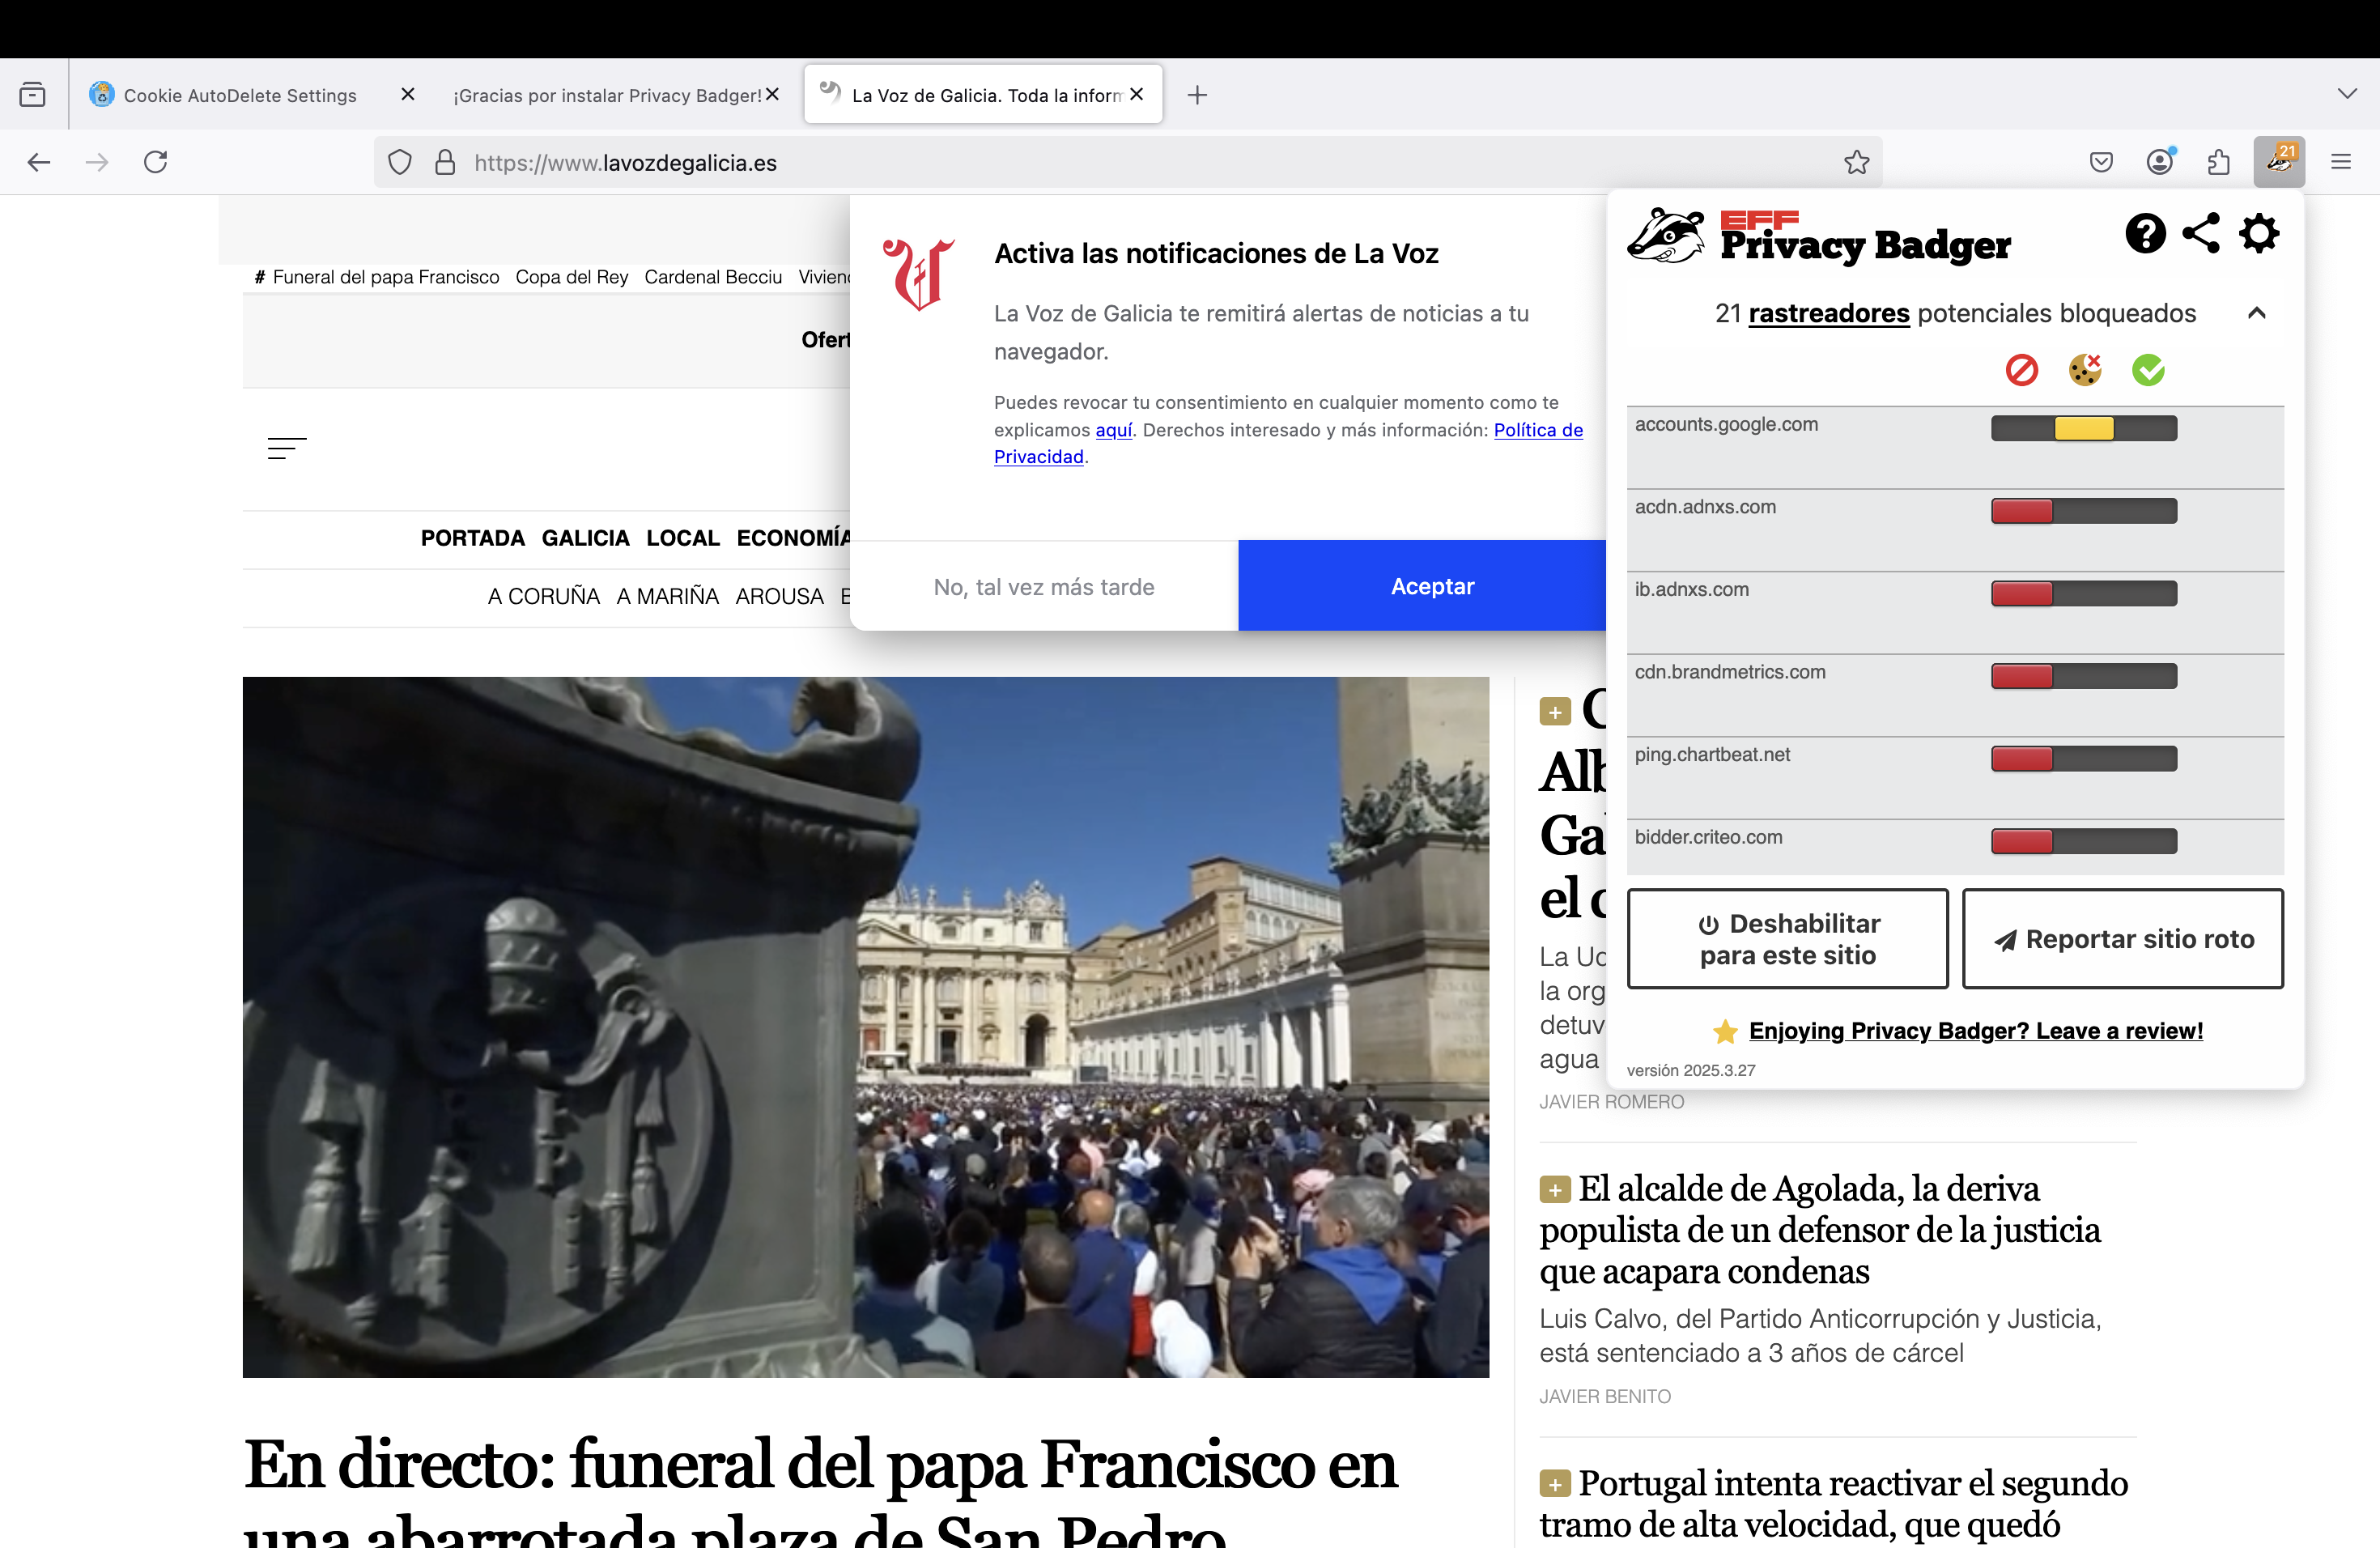
\includegraphics[width=\textwidth]{resultado_privacybadger.png}
    \caption{Resultado Privacy Badger}
    \label{fig:resultado_privacybadger}
\end{figure}
